\documentclass[twoside]{book}

% Packages required by doxygen
\usepackage{fixltx2e}
\usepackage{calc}
\usepackage{doxygen}
\usepackage[export]{adjustbox} % also loads graphicx
\usepackage{graphicx}
\usepackage[utf8]{inputenc}
\usepackage{makeidx}
\usepackage{multicol}
\usepackage{multirow}
\PassOptionsToPackage{warn}{textcomp}
\usepackage{textcomp}
\usepackage[nointegrals]{wasysym}
\usepackage[table]{xcolor}

% NLS support packages
\usepackage[T2A]{fontenc}
\usepackage[russian]{babel}

% Font selection
\usepackage[T1]{fontenc}
\usepackage[scaled=.90]{helvet}
\usepackage{courier}
\usepackage{amssymb}
\usepackage{sectsty}
\renewcommand{\familydefault}{\sfdefault}
\allsectionsfont{%
  \fontseries{bc}\selectfont%
  \color{darkgray}%
}
\renewcommand{\DoxyLabelFont}{%
  \fontseries{bc}\selectfont%
  \color{darkgray}%
}
\newcommand{\+}{\discretionary{\mbox{\scriptsize$\hookleftarrow$}}{}{}}

% Page & text layout
\usepackage{geometry}
\geometry{%
  a4paper,%
  top=2.5cm,%
  bottom=2.5cm,%
  left=2.5cm,%
  right=2.5cm%
}
\tolerance=750
\hfuzz=15pt
\hbadness=750
\setlength{\emergencystretch}{15pt}
\setlength{\parindent}{0cm}
\setlength{\parskip}{0.2cm}
\makeatletter
\renewcommand{\paragraph}{%
  \@startsection{paragraph}{4}{0ex}{-1.0ex}{1.0ex}{%
    \normalfont\normalsize\bfseries\SS@parafont%
  }%
}
\renewcommand{\subparagraph}{%
  \@startsection{subparagraph}{5}{0ex}{-1.0ex}{1.0ex}{%
    \normalfont\normalsize\bfseries\SS@subparafont%
  }%
}
\makeatother

% Headers & footers
\usepackage{fancyhdr}
\pagestyle{fancyplain}
\fancyhead[LE]{\fancyplain{}{\bfseries\thepage}}
\fancyhead[CE]{\fancyplain{}{}}
\fancyhead[RE]{\fancyplain{}{\bfseries\leftmark}}
\fancyhead[LO]{\fancyplain{}{\bfseries\rightmark}}
\fancyhead[CO]{\fancyplain{}{}}
\fancyhead[RO]{\fancyplain{}{\bfseries\thepage}}
\fancyfoot[LE]{\fancyplain{}{}}
\fancyfoot[CE]{\fancyplain{}{}}
\fancyfoot[RE]{\fancyplain{}{\bfseries\scriptsize Документация по q\+Chess. Последние изменения\+: Вт 28 Июл 2015 16\+:58\+:13. Создано системой Doxygen }}
\fancyfoot[LO]{\fancyplain{}{\bfseries\scriptsize Документация по q\+Chess. Последние изменения\+: Вт 28 Июл 2015 16\+:58\+:13. Создано системой Doxygen }}
\fancyfoot[CO]{\fancyplain{}{}}
\fancyfoot[RO]{\fancyplain{}{}}
\renewcommand{\footrulewidth}{0.4pt}
\renewcommand{\chaptermark}[1]{%
  \markboth{#1}{}%
}
\renewcommand{\sectionmark}[1]{%
  \markright{\thesection\ #1}%
}

% Indices & bibliography
\usepackage{natbib}
\usepackage[titles]{tocloft}
\setcounter{tocdepth}{3}
\setcounter{secnumdepth}{5}
\makeindex

% Hyperlinks (required, but should be loaded last)
\usepackage{ifpdf}
\ifpdf
  \usepackage[pdftex,pagebackref=true]{hyperref}
\else
  \usepackage[ps2pdf,pagebackref=true]{hyperref}
\fi
\hypersetup{%
  colorlinks=true,%
  linkcolor=blue,%
  citecolor=blue,%
  unicode%
}

% Custom commands
\newcommand{\clearemptydoublepage}{%
  \newpage{\pagestyle{empty}\cleardoublepage}%
}


%===== C O N T E N T S =====

\begin{document}

% Titlepage & ToC
\hypersetup{pageanchor=false,
             bookmarks=true,
             bookmarksnumbered=true,
             pdfencoding=unicode
            }
\pagenumbering{roman}
\begin{titlepage}
\vspace*{7cm}
\begin{center}%
{\Large q\+Chess \\[1ex]\large 0.\+1a }\\
\vspace*{1cm}
{\large Создано системой Doxygen 1.8.9.1}\\
\vspace*{0.5cm}
{\small Вт 28 Июл 2015 16:58:13}\\
\end{center}
\end{titlepage}
\clearemptydoublepage
\tableofcontents
\clearemptydoublepage
\pagenumbering{arabic}
\hypersetup{pageanchor=true}

%--- Begin generated contents ---
\chapter{q\+Chess -\/ разработано в рамках летней практики ВолгГТУ ПОАС 2015.}
\label{md__r_e_a_d_m_e}
\hypertarget{md__r_e_a_d_m_e}{}
\input{md__r_e_a_d_m_e}
\chapter{Иерархический список классов}
\section{Иерархия классов}
Иерархия классов.\begin{DoxyCompactList}
\item \contentsline{section}{bit\+Board}{\pageref{classbit_board}}{}
\item \contentsline{section}{board}{\pageref{classboard}}{}
\item \contentsline{section}{board\+Move}{\pageref{classboard_move}}{}
\item \contentsline{section}{board\+Position}{\pageref{classboard_position}}{}
\item \contentsline{section}{chess\+Game\+State}{\pageref{classchess_game_state}}{}
\item \contentsline{section}{chess\+Player}{\pageref{classchess_player}}{}
\begin{DoxyCompactList}
\item \contentsline{section}{A\+I}{\pageref{class_a_i}}{}
\item \contentsline{section}{human}{\pageref{classhuman}}{}
\end{DoxyCompactList}
\item \contentsline{section}{options}{\pageref{classoptions}}{}
\item \contentsline{section}{piece}{\pageref{classpiece}}{}
\item \contentsline{section}{piece\+Set}{\pageref{classpiece_set}}{}
\item Q\+Object\begin{DoxyCompactList}
\item \contentsline{section}{chess\+Game}{\pageref{classchess_game}}{}
\end{DoxyCompactList}
\item \contentsline{section}{serial\+Board}{\pageref{structserial_board}}{}
\item \contentsline{section}{stat\+Snapshot}{\pageref{classstat_snapshot}}{}
\end{DoxyCompactList}

\chapter{Алфавитный указатель классов}
\section{Классы}
Классы с их кратким описанием.\begin{DoxyCompactList}
\item\contentsline{section}{\hyperlink{class_a_i}{A\+I} \\*
\begin{DoxyItemize}
\item описывает игрока искуственного интелекта 
\end{DoxyItemize}}{\pageref{class_a_i}}{}
\item\contentsline{section}{\hyperlink{classbit_board}{bit\+Board} \\*
\begin{DoxyItemize}
\item побитовая карта доски. (т.\+к. тип unsigned long long содержит 64 бита, что равно кол ву полей на доске) 
\end{DoxyItemize}}{\pageref{classbit_board}}{}
\item\contentsline{section}{\hyperlink{classboard}{board} }{\pageref{classboard}}{}
\item\contentsline{section}{\hyperlink{classboard_move}{board\+Move} \\*
\begin{DoxyItemize}
\item класс игрового хода 
\end{DoxyItemize}}{\pageref{classboard_move}}{}
\item\contentsline{section}{\hyperlink{classboard_position}{board\+Position} \\*
\begin{DoxyItemize}
\item класс которы описывает позицию на доске 
\end{DoxyItemize}}{\pageref{classboard_position}}{}
\item\contentsline{section}{\hyperlink{classchess_game}{chess\+Game} \\*
\begin{DoxyItemize}
\item класс партии 
\end{DoxyItemize}}{\pageref{classchess_game}}{}
\item\contentsline{section}{\hyperlink{classchess_game_state}{chess\+Game\+State} \\*
\begin{DoxyItemize}
\item класс описывающий игровое соостояние 
\end{DoxyItemize}}{\pageref{classchess_game_state}}{}
\item\contentsline{section}{\hyperlink{classchess_player}{chess\+Player} \\*
\begin{DoxyItemize}
\item абстрактный класс игрока 
\end{DoxyItemize}}{\pageref{classchess_player}}{}
\item\contentsline{section}{\hyperlink{classhuman}{human} \\*
\begin{DoxyItemize}
\item описывает игрока человека 
\end{DoxyItemize}}{\pageref{classhuman}}{}
\item\contentsline{section}{\hyperlink{classoptions}{options} \\*
\begin{DoxyItemize}
\item класс конфигураций (содержит все конфигурации программы) 
\end{DoxyItemize}}{\pageref{classoptions}}{}
\item\contentsline{section}{\hyperlink{classpiece}{piece} \\*
\begin{DoxyItemize}
\item класс шахматной фигуры 
\end{DoxyItemize}}{\pageref{classpiece}}{}
\item\contentsline{section}{\hyperlink{classpiece_set}{piece\+Set} }{\pageref{classpiece_set}}{}
\item\contentsline{section}{\hyperlink{structserial_board}{serial\+Board} \\*The \hyperlink{structserial_board}{serial\+Board} struct -\/ упращенная структура представления доски }{\pageref{structserial_board}}{}
\item\contentsline{section}{\hyperlink{classstat_snapshot}{stat\+Snapshot} }{\pageref{classstat_snapshot}}{}
\end{DoxyCompactList}

\chapter{Классы}
\hypertarget{class_a_i}{}\section{Класс A\+I}
\label{class_a_i}\index{A\+I@{A\+I}}


The \hyperlink{class_a_i}{A\+I} class -\/ описывает игрока искуственного интелекта  




{\ttfamily \#include $<$chessplayer.\+h$>$}

Граф наследования\+:A\+I\+:\begin{figure}[H]
\begin{center}
\leavevmode
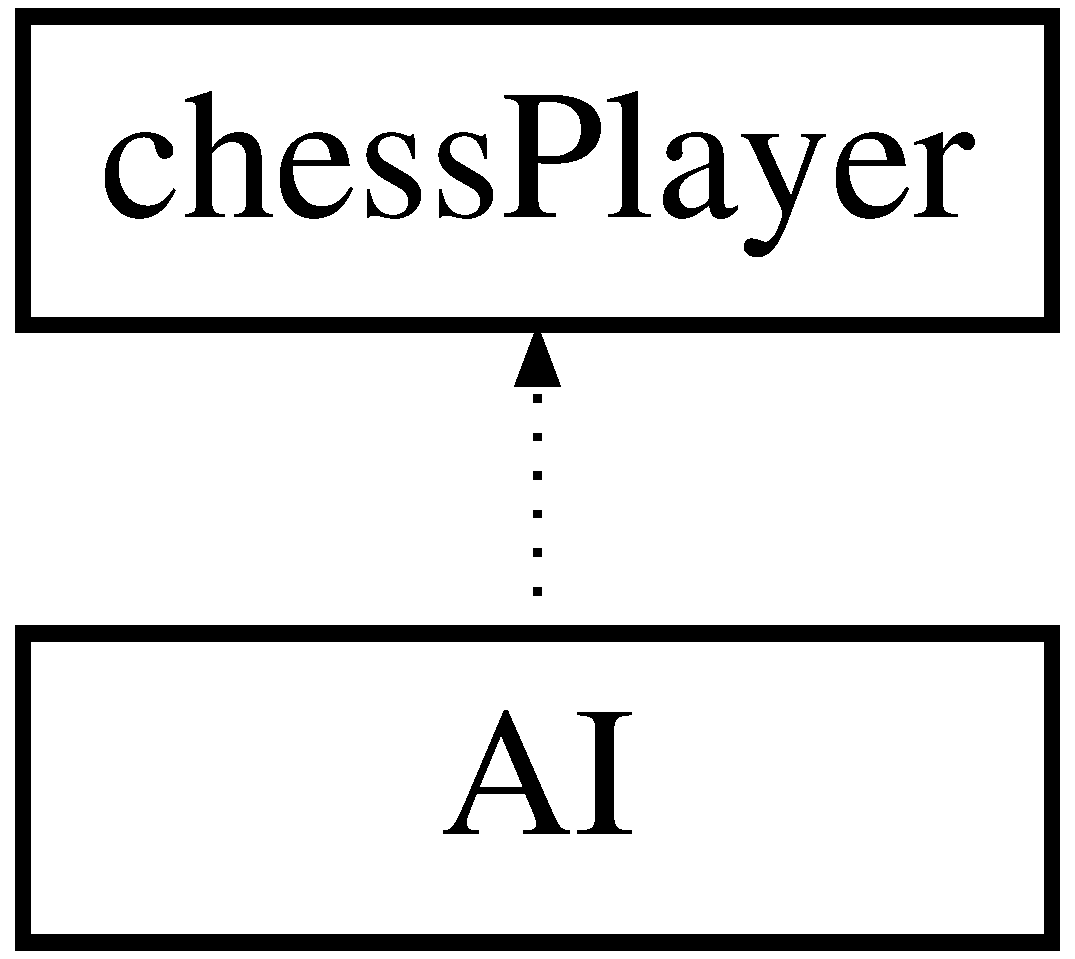
\includegraphics[height=2.000000cm]{class_a_i}
\end{center}
\end{figure}
\subsection*{Открытые члены}
\begin{DoxyCompactItemize}
\item 
\hypertarget{class_a_i_a6cda26d3bf7238b1a7ea3725bf4aabb7}{}virtual void {\bfseries new\+Game} ()\label{class_a_i_a6cda26d3bf7238b1a7ea3725bf4aabb7}

\item 
\hypertarget{class_a_i_a522cd4b638779e79a22bdca7c720117e}{}virtual void {\bfseries start\+Game} ()\label{class_a_i_a522cd4b638779e79a22bdca7c720117e}

\item 
\hypertarget{class_a_i_aa8be74c446a6c45782b751603eacfc9c}{}virtual void {\bfseries load\+Game} (const \hyperlink{classchess_game_state}{chess\+Game\+State} \&cgs)\label{class_a_i_aa8be74c446a6c45782b751603eacfc9c}

\item 
\hypertarget{class_a_i_a86e46248e15fae19e4e12905f2b57f29}{}virtual void {\bfseries opponent\+Move} (const \hyperlink{classboard_move}{board\+Move} \&move, const \hyperlink{classchess_game_state}{chess\+Game\+State} \&cgs)\label{class_a_i_a86e46248e15fae19e4e12905f2b57f29}

\item 
\hypertarget{class_a_i_a2f3438ffaf88c009c07fee1839fabd05}{}virtual void {\bfseries think} (const \hyperlink{classchess_game_state}{chess\+Game\+State} \&cgs)\label{class_a_i_a2f3438ffaf88c009c07fee1839fabd05}

\item 
\hypertarget{class_a_i_a4e39220413e38cc5ab65c127422cd5b1}{}virtual bool {\bfseries need\+Move} ()\label{class_a_i_a4e39220413e38cc5ab65c127422cd5b1}

\item 
\hypertarget{class_a_i_a7b9d1d6efcece382034e191ed9a6ed78}{}virtual void {\bfseries undo\+Move} ()\label{class_a_i_a7b9d1d6efcece382034e191ed9a6ed78}

\item 
\hypertarget{class_a_i_ad77351f99c6ad80f9d675b9affec7f44}{}int {\bfseries get\+Ply} ()\label{class_a_i_ad77351f99c6ad80f9d675b9affec7f44}

\item 
\hypertarget{class_a_i_a28d820a70a78d7ce290179c10a869c78}{}void {\bfseries set\+Ply} (int ply)\label{class_a_i_a28d820a70a78d7ce290179c10a869c78}

\end{DoxyCompactItemize}
\subsection*{Защищенные члены}
\begin{DoxyCompactItemize}
\item 
\hypertarget{class_a_i_a1c6741642292f898fdf8d7ce6c13683f}{}int {\bfseries evaluate\+Board} (const \hyperlink{classboard}{board} \&b, \hyperlink{classpiece_a0e121e5952345fd0e7014a8e6a1fbbda}{piece\+::color} c)\label{class_a_i_a1c6741642292f898fdf8d7ce6c13683f}

\item 
\hypertarget{class_a_i_ad66d3b4e9d52d3025d3e043cb90dfd3e}{}int {\bfseries search} (\hyperlink{classboard}{board} b, \hyperlink{classpiece_a0e121e5952345fd0e7014a8e6a1fbbda}{piece\+::color} c, int depth, int alpha, int beta, \hyperlink{classboard_move}{board\+Move} \&bm)\label{class_a_i_ad66d3b4e9d52d3025d3e043cb90dfd3e}

\item 
\hypertarget{class_a_i_a748a22bb7df0c157ac1db36d1357a749}{}int {\bfseries pawn\+Bonus} (const \hyperlink{classboard_position}{board\+Position} \&bp, const \hyperlink{classboard}{board} \&b, \hyperlink{classpiece_a0e121e5952345fd0e7014a8e6a1fbbda}{piece\+::color} turn, bool endgame)\label{class_a_i_a748a22bb7df0c157ac1db36d1357a749}

\item 
\hypertarget{class_a_i_a27427ae20aa7eb46effbd28fc29917e7}{}int {\bfseries knight\+Bonus} (const \hyperlink{classboard_position}{board\+Position} \&bp, const \hyperlink{classboard}{board} \&b, \hyperlink{classpiece_a0e121e5952345fd0e7014a8e6a1fbbda}{piece\+::color} turn, bool endgame)\label{class_a_i_a27427ae20aa7eb46effbd28fc29917e7}

\item 
\hypertarget{class_a_i_a1c5a4f19af6bc2d2827db4c7df4b0927}{}int {\bfseries bishop\+Bonus} (const \hyperlink{classboard_position}{board\+Position} \&bp, const \hyperlink{classboard}{board} \&b, \hyperlink{classpiece_a0e121e5952345fd0e7014a8e6a1fbbda}{piece\+::color} turn, bool endgame)\label{class_a_i_a1c5a4f19af6bc2d2827db4c7df4b0927}

\item 
\hypertarget{class_a_i_af25d9b4511e7c435c9593ca2c1f3335d}{}int {\bfseries rook\+Bonus} (const \hyperlink{classboard_position}{board\+Position} \&bp, const \hyperlink{classboard}{board} \&b, \hyperlink{classpiece_a0e121e5952345fd0e7014a8e6a1fbbda}{piece\+::color} turn, bool endgame)\label{class_a_i_af25d9b4511e7c435c9593ca2c1f3335d}

\item 
\hypertarget{class_a_i_ada53e6fb423614dc425d33ae7f2f0dcf}{}int {\bfseries queen\+Bonus} (const \hyperlink{classboard_position}{board\+Position} \&bp, const \hyperlink{classboard}{board} \&b, \hyperlink{classpiece_a0e121e5952345fd0e7014a8e6a1fbbda}{piece\+::color} turn, bool endgame)\label{class_a_i_ada53e6fb423614dc425d33ae7f2f0dcf}

\item 
\hypertarget{class_a_i_aa6c91d60f9d36a1edafadfb84b67baf5}{}int {\bfseries king\+Bonus} (const \hyperlink{classboard_position}{board\+Position} \&bp, const \hyperlink{classboard}{board} \&b, \hyperlink{classpiece_a0e121e5952345fd0e7014a8e6a1fbbda}{piece\+::color} turn, bool endgame)\label{class_a_i_aa6c91d60f9d36a1edafadfb84b67baf5}

\item 
\hypertarget{class_a_i_ab019ac70f41b6fc7a477286d3d65b9da}{}int {\bfseries num\+Attacked\+Squares} (const mask \&piece\+Attacks)\label{class_a_i_ab019ac70f41b6fc7a477286d3d65b9da}

\item 
\hypertarget{class_a_i_a320ff94f5b15c0ed83ba704326ca23d3}{}bool {\bfseries is\+Isolated\+Pawn} (const \hyperlink{classboard_position}{board\+Position} \&bp, const \hyperlink{classboard}{board} \&b)\label{class_a_i_a320ff94f5b15c0ed83ba704326ca23d3}

\item 
\hypertarget{class_a_i_acd477b147adb58a9878b3c1499bf6ea1}{}bool {\bfseries is\+Doubled\+Pawn} (const \hyperlink{classboard_position}{board\+Position} \&bp, const \hyperlink{classboard}{board} \&b)\label{class_a_i_acd477b147adb58a9878b3c1499bf6ea1}

\end{DoxyCompactItemize}
\subsection*{Защищенные данные}
\begin{DoxyCompactItemize}
\item 
\hypertarget{class_a_i_a38e07f36c7574a06bf5e1001283fe404}{}int {\bfseries l\+Ply}\label{class_a_i_a38e07f36c7574a06bf5e1001283fe404}

\end{DoxyCompactItemize}
\subsection*{Статические защищенные данные}
\begin{DoxyCompactItemize}
\item 
static int {\bfseries m\+\_\+bishop} \mbox{[}64\mbox{]}
\item 
static int {\bfseries m\+\_\+knight} \mbox{[}64\mbox{]}
\item 
static int {\bfseries m\+\_\+wpawn} \mbox{[}64\mbox{]}
\item 
static int {\bfseries m\+\_\+bpawn} \mbox{[}64\mbox{]}
\item 
static int {\bfseries m\+\_\+wking} \mbox{[}64\mbox{]}
\item 
static int {\bfseries m\+\_\+bking} \mbox{[}64\mbox{]}
\item 
static int {\bfseries m\+\_\+end\+\_\+king} \mbox{[}64\mbox{]}
\end{DoxyCompactItemize}


\subsection{Подробное описание}
The \hyperlink{class_a_i}{A\+I} class -\/ описывает игрока искуственного интелекта 

\subsection{Данные класса}
\hypertarget{class_a_i_ab749c006dc52480c5a9a00d17318e533}{}\index{A\+I@{A\+I}!m\+\_\+bishop@{m\+\_\+bishop}}
\index{m\+\_\+bishop@{m\+\_\+bishop}!A\+I@{A\+I}}
\subsubsection[{m\+\_\+bishop}]{\setlength{\rightskip}{0pt plus 5cm}int A\+I\+::m\+\_\+bishop\hspace{0.3cm}{\ttfamily [static]}, {\ttfamily [protected]}}\label{class_a_i_ab749c006dc52480c5a9a00d17318e533}
{\bfseries Инициализатор}
\begin{DoxyCode}
= \{
    -5,-5,-5,-5,-5,-5,-5,-5,
    -5,10,5,10,10,5,10,-5,
    -5,5,3,12,12,3,5,-5,
    -5,3,12,3,3,12,3,-5,
    -5,3,12,3,3,12,3,-5,
    -5,5,3,12,12,3,5,-5,
    -5,10,5,10,10,5,10,-5,
    -5,-5,-5,-5,-5,-5,-5,-5 \}
\end{DoxyCode}
\hypertarget{class_a_i_a816338121fb591918d66bdefb4cda805}{}\index{A\+I@{A\+I}!m\+\_\+bking@{m\+\_\+bking}}
\index{m\+\_\+bking@{m\+\_\+bking}!A\+I@{A\+I}}
\subsubsection[{m\+\_\+bking}]{\setlength{\rightskip}{0pt plus 5cm}int A\+I\+::m\+\_\+bking\hspace{0.3cm}{\ttfamily [static]}, {\ttfamily [protected]}}\label{class_a_i_a816338121fb591918d66bdefb4cda805}
{\bfseries Инициализатор}
\begin{DoxyCode}
= \{
    -55,-55,-89,-89,-89,-89,-55,-55,
    -34,-34,-55,-55,-55,-55,-34,-34,
    -21,-21,-34,-34,-34,-34,-21,-21,
    -13,-13,-21,-21,-21,-21,-13,-13,
    -8,-8,-13,-13,-13,-13,-8,-8,
    -5,-5,-8,-8,-8,-8,-5,-5,
    -3,-3,-5,-5,-5,-5,-3,-3,
    2,10,4,0,0,7,10,2\}
\end{DoxyCode}
\hypertarget{class_a_i_aed628e02e8d5bdc970bfb01acd6162f2}{}\index{A\+I@{A\+I}!m\+\_\+bpawn@{m\+\_\+bpawn}}
\index{m\+\_\+bpawn@{m\+\_\+bpawn}!A\+I@{A\+I}}
\subsubsection[{m\+\_\+bpawn}]{\setlength{\rightskip}{0pt plus 5cm}int A\+I\+::m\+\_\+bpawn\hspace{0.3cm}{\ttfamily [static]}, {\ttfamily [protected]}}\label{class_a_i_aed628e02e8d5bdc970bfb01acd6162f2}
{\bfseries Инициализатор}
\begin{DoxyCode}
= \{
    0,0,0,0,0,0,0,0,
    5,10,15,20,20,15,10,5,
    4,8,12,16,16,12,8,4,
    3,6,9,12,12,9,6,3,
    2,4,6,8,8,6,4,2,
    1,2,3,4,4,3,2,1,
    0,0,0,-5,-5,0,0,0,
    0,0,0,0,0,0,0,0 \}
\end{DoxyCode}
\hypertarget{class_a_i_aa578831d72d1539297b700dd5c6b37d6}{}\index{A\+I@{A\+I}!m\+\_\+end\+\_\+king@{m\+\_\+end\+\_\+king}}
\index{m\+\_\+end\+\_\+king@{m\+\_\+end\+\_\+king}!A\+I@{A\+I}}
\subsubsection[{m\+\_\+end\+\_\+king}]{\setlength{\rightskip}{0pt plus 5cm}int A\+I\+::m\+\_\+end\+\_\+king\hspace{0.3cm}{\ttfamily [static]}, {\ttfamily [protected]}}\label{class_a_i_aa578831d72d1539297b700dd5c6b37d6}
{\bfseries Инициализатор}
\begin{DoxyCode}
= \{
    -5,-3,-1,0,0,-1,-3,-5,
    -3,5,5,5,5,5,5,-3,
    -1,5,10,10,10,10,5,-1,
    0,5,10,15,15,10,5,0,
    0,5,10,15,15,10,5,0,
    -1,5,10,10,10,10,5,-1,
    -3,5,5,5,5,5,5,-3,
    -5,-3,-1,0,0,-1,-3,-5\}
\end{DoxyCode}
\hypertarget{class_a_i_adbe96956dc1a50f47c828c04072cecfe}{}\index{A\+I@{A\+I}!m\+\_\+knight@{m\+\_\+knight}}
\index{m\+\_\+knight@{m\+\_\+knight}!A\+I@{A\+I}}
\subsubsection[{m\+\_\+knight}]{\setlength{\rightskip}{0pt plus 5cm}int A\+I\+::m\+\_\+knight\hspace{0.3cm}{\ttfamily [static]}, {\ttfamily [protected]}}\label{class_a_i_adbe96956dc1a50f47c828c04072cecfe}
{\bfseries Инициализатор}
\begin{DoxyCode}
= \{
    -10,-5,-5,-5,-5,-5,-5,-10,
    -5,0,0,3,3,0,0,-5,
    -5,0,5,5,5,5,0,-5,
    -5,0,5,10,10,5,0,-5,
    -5,0,5,10,10,5,0,-5,
    -5,0,5,5,5,5,0,-5,
    -5,0,0,3,3,0,0,-5,
    -10,-5,-5,-5,-5,-5,-5,-10 \}
\end{DoxyCode}
\hypertarget{class_a_i_ac30650d294d82469e1c869e76ee7986f}{}\index{A\+I@{A\+I}!m\+\_\+wking@{m\+\_\+wking}}
\index{m\+\_\+wking@{m\+\_\+wking}!A\+I@{A\+I}}
\subsubsection[{m\+\_\+wking}]{\setlength{\rightskip}{0pt plus 5cm}int A\+I\+::m\+\_\+wking\hspace{0.3cm}{\ttfamily [static]}, {\ttfamily [protected]}}\label{class_a_i_ac30650d294d82469e1c869e76ee7986f}
{\bfseries Инициализатор}
\begin{DoxyCode}
= \{
    2,10,4,0,0,7,10,2,
    -3,-3,-5,-5,-5,-5,-3,-3,
    -5,-5,-8,-8,-8,-8,-5,-5,
    -8,-8,-13,-13,-13,-13,-8,-8,
    -13,-13,-21,-21,-21,-21,-13,-13,
    -21,-21,-34,-34,-34,-34,-21,-21,
    -34,-34,-55,-55,-55,-55,-34,-34,
    -55,-55,-89,-89,-89,-89,-55,-55\}
\end{DoxyCode}
\hypertarget{class_a_i_afc5127e7859211a872a6df3fdbe971d0}{}\index{A\+I@{A\+I}!m\+\_\+wpawn@{m\+\_\+wpawn}}
\index{m\+\_\+wpawn@{m\+\_\+wpawn}!A\+I@{A\+I}}
\subsubsection[{m\+\_\+wpawn}]{\setlength{\rightskip}{0pt plus 5cm}int A\+I\+::m\+\_\+wpawn\hspace{0.3cm}{\ttfamily [static]}, {\ttfamily [protected]}}\label{class_a_i_afc5127e7859211a872a6df3fdbe971d0}
{\bfseries Инициализатор}
\begin{DoxyCode}
= \{
    0,0,0,0,0,0,0,0,
    0,0,0,-5,-5,0,0,0,
    1,2,3,4,4,3,2,1,
    2,4,6,8,8,6,4,2,
    3,6,9,12,12,9,6,3,
    4,8,12,16,16,12,8,4,
    5,10,15,20,20,15,10,5,
    0,0,0,0,0,0,0,0 \}
\end{DoxyCode}


Объявления и описания членов классов находятся в файлах\+:\begin{DoxyCompactItemize}
\item 
Model/chessplayer.\+h\item 
Model/chessplayer.\+cpp\end{DoxyCompactItemize}

\hypertarget{classbit_board}{}\section{Класс bit\+Board}
\label{classbit_board}\index{bit\+Board@{bit\+Board}}


The \hyperlink{classbit_board}{bit\+Board} class -\/ побитовая карта доски. (т.\+к. тип unsigned long long содержит 64 бита, что равно кол ву полей на доске)  




{\ttfamily \#include $<$bitboard.\+h$>$}

\subsection*{Открытые члены}
\begin{DoxyCompactItemize}
\item 
\hypertarget{classbit_board_a1da2ef5a1d5e5ceb731dd5b7fbbbf386}{}\hyperlink{classbit_board_a1da2ef5a1d5e5ceb731dd5b7fbbbf386}{bit\+Board} ()\label{classbit_board_a1da2ef5a1d5e5ceb731dd5b7fbbbf386}

\begin{DoxyCompactList}\small\item\em \hyperlink{classbit_board}{bit\+Board} -\/ конструктор в результате которого все биты опущены \end{DoxyCompactList}\item 
\hyperlink{classbit_board_abac32dec74ed2dd32995955a07422198}{bit\+Board} (const unsigned long long \&\hyperlink{classboard}{board})
\begin{DoxyCompactList}\small\item\em \hyperlink{classbit_board}{bit\+Board} -\/ конструктор который копирует исходную битовую маску \end{DoxyCompactList}\item 
void \hyperlink{classbit_board_a3ec51b1e23ec2a8903c7f9fbf7e79889}{set\+Bit} (const \hyperlink{classboard_position}{board\+Position} \&bp)
\begin{DoxyCompactList}\small\item\em set\+Bit -\/ устанавливает бит в заданной позиции в поднятое положение \end{DoxyCompactList}\item 
void \hyperlink{classbit_board_a931987de9741781789d2dd20bd9aef62}{unset\+Bit} (const \hyperlink{classboard_position}{board\+Position} \&bp)
\begin{DoxyCompactList}\small\item\em unset\+Bit -\/ устанавливает бит в заданной позиции в опущенное положение \end{DoxyCompactList}\item 
\hypertarget{classbit_board_af8359ea0e11d66aa70667a521569c6f0}{}void \hyperlink{classbit_board_af8359ea0e11d66aa70667a521569c6f0}{invert} ()\label{classbit_board_af8359ea0e11d66aa70667a521569c6f0}

\begin{DoxyCompactList}\small\item\em invert -\/ переворачивает все биты доски \end{DoxyCompactList}\item 
unsigned long long \hyperlink{classbit_board_afe3388c61bf3046f85ce48f287f2d912}{get\+Board} () const 
\begin{DoxyCompactList}\small\item\em get\+Board -\/ вернуть битовую маску \end{DoxyCompactList}\end{DoxyCompactItemize}
\subsection*{Открытые статические члены}
\begin{DoxyCompactItemize}
\item 
static unsigned long long \hyperlink{classbit_board_a31dd95717cbb107a4fe6d334407dfd4e}{get\+X\+Mask} (const \hyperlink{classboard_position}{board\+Position} \&bp)
\begin{DoxyCompactList}\small\item\em get\+X\+Mask -\/ вернет все битовую маску для всех позицы с координатой х равной bp.\+x() \end{DoxyCompactList}\item 
static unsigned long long \hyperlink{classbit_board_acc9d2cf1cd3af85481f5a26ffc656794}{get\+Y\+Mask} (const \hyperlink{classboard_position}{board\+Position} \&bp)
\begin{DoxyCompactList}\small\item\em get\+Y\+Mask -\/ вернет все битовую маску для всех позицы с координатой y равной bp.\+x() \end{DoxyCompactList}\item 
static unsigned long long \hyperlink{classbit_board_a2476b527524fbf53a6c55554e1225b76}{get\+Mask} (const \hyperlink{classboard_position}{board\+Position} \&bp)
\begin{DoxyCompactList}\small\item\em get\+Mask -\/ возвращает маску заданного бита \end{DoxyCompactList}\end{DoxyCompactItemize}


\subsection{Подробное описание}
The \hyperlink{classbit_board}{bit\+Board} class -\/ побитовая карта доски. (т.\+к. тип unsigned long long содержит 64 бита, что равно кол ву полей на доске) 

\subsection{Конструктор(ы)}
\hypertarget{classbit_board_abac32dec74ed2dd32995955a07422198}{}\index{bit\+Board@{bit\+Board}!bit\+Board@{bit\+Board}}
\index{bit\+Board@{bit\+Board}!bit\+Board@{bit\+Board}}
\subsubsection[{bit\+Board}]{\setlength{\rightskip}{0pt plus 5cm}bit\+Board\+::bit\+Board (
\begin{DoxyParamCaption}
\item[{const unsigned long long \&}]{board}
\end{DoxyParamCaption}
)}\label{classbit_board_abac32dec74ed2dd32995955a07422198}


\hyperlink{classbit_board}{bit\+Board} -\/ конструктор который копирует исходную битовую маску 


\begin{DoxyParams}{Аргументы}
{\em board} & -\/ битовая маска \\
\hline
\end{DoxyParams}


\subsection{Методы}
\hypertarget{classbit_board_afe3388c61bf3046f85ce48f287f2d912}{}\index{bit\+Board@{bit\+Board}!get\+Board@{get\+Board}}
\index{get\+Board@{get\+Board}!bit\+Board@{bit\+Board}}
\subsubsection[{get\+Board}]{\setlength{\rightskip}{0pt plus 5cm}unsigned long long bit\+Board\+::get\+Board (
\begin{DoxyParamCaption}
{}
\end{DoxyParamCaption}
) const\hspace{0.3cm}{\ttfamily [inline]}}\label{classbit_board_afe3388c61bf3046f85ce48f287f2d912}


get\+Board -\/ вернуть битовую маску 

\begin{DoxyReturn}{Возвращает}
-\/ битовая маска 
\end{DoxyReturn}
\hypertarget{classbit_board_a2476b527524fbf53a6c55554e1225b76}{}\index{bit\+Board@{bit\+Board}!get\+Mask@{get\+Mask}}
\index{get\+Mask@{get\+Mask}!bit\+Board@{bit\+Board}}
\subsubsection[{get\+Mask}]{\setlength{\rightskip}{0pt plus 5cm}unsigned long long bit\+Board\+::get\+Mask (
\begin{DoxyParamCaption}
\item[{const {\bf board\+Position} \&}]{bp}
\end{DoxyParamCaption}
)\hspace{0.3cm}{\ttfamily [static]}}\label{classbit_board_a2476b527524fbf53a6c55554e1225b76}


get\+Mask -\/ возвращает маску заданного бита 


\begin{DoxyParams}{Аргументы}
{\em bp} & -\/ позиция бита \\
\hline
\end{DoxyParams}
\begin{DoxyReturn}{Возвращает}
маска где понят или опущен необходимый бит, остальные опущены 
\end{DoxyReturn}
\hypertarget{classbit_board_a31dd95717cbb107a4fe6d334407dfd4e}{}\index{bit\+Board@{bit\+Board}!get\+X\+Mask@{get\+X\+Mask}}
\index{get\+X\+Mask@{get\+X\+Mask}!bit\+Board@{bit\+Board}}
\subsubsection[{get\+X\+Mask}]{\setlength{\rightskip}{0pt plus 5cm}unsigned long long bit\+Board\+::get\+X\+Mask (
\begin{DoxyParamCaption}
\item[{const {\bf board\+Position} \&}]{bp}
\end{DoxyParamCaption}
)\hspace{0.3cm}{\ttfamily [static]}}\label{classbit_board_a31dd95717cbb107a4fe6d334407dfd4e}


get\+X\+Mask -\/ вернет все битовую маску для всех позицы с координатой х равной bp.\+x() 


\begin{DoxyParams}{Аргументы}
{\em bp} & -\/ текущая позиция \\
\hline
\end{DoxyParams}
\begin{DoxyReturn}{Возвращает}
-\/ битовая маска 
\end{DoxyReturn}
\hypertarget{classbit_board_acc9d2cf1cd3af85481f5a26ffc656794}{}\index{bit\+Board@{bit\+Board}!get\+Y\+Mask@{get\+Y\+Mask}}
\index{get\+Y\+Mask@{get\+Y\+Mask}!bit\+Board@{bit\+Board}}
\subsubsection[{get\+Y\+Mask}]{\setlength{\rightskip}{0pt plus 5cm}unsigned long long bit\+Board\+::get\+Y\+Mask (
\begin{DoxyParamCaption}
\item[{const {\bf board\+Position} \&}]{bp}
\end{DoxyParamCaption}
)\hspace{0.3cm}{\ttfamily [static]}}\label{classbit_board_acc9d2cf1cd3af85481f5a26ffc656794}


get\+Y\+Mask -\/ вернет все битовую маску для всех позицы с координатой y равной bp.\+x() 


\begin{DoxyParams}{Аргументы}
{\em bp} & -\/ текущая позиция \\
\hline
\end{DoxyParams}
\begin{DoxyReturn}{Возвращает}
-\/ битовая маска 
\end{DoxyReturn}
\hypertarget{classbit_board_a3ec51b1e23ec2a8903c7f9fbf7e79889}{}\index{bit\+Board@{bit\+Board}!set\+Bit@{set\+Bit}}
\index{set\+Bit@{set\+Bit}!bit\+Board@{bit\+Board}}
\subsubsection[{set\+Bit}]{\setlength{\rightskip}{0pt plus 5cm}void bit\+Board\+::set\+Bit (
\begin{DoxyParamCaption}
\item[{const {\bf board\+Position} \&}]{bp}
\end{DoxyParamCaption}
)}\label{classbit_board_a3ec51b1e23ec2a8903c7f9fbf7e79889}


set\+Bit -\/ устанавливает бит в заданной позиции в поднятое положение 


\begin{DoxyParams}{Аргументы}
{\em bp} & -\/ позиция \\
\hline
\end{DoxyParams}
\hypertarget{classbit_board_a931987de9741781789d2dd20bd9aef62}{}\index{bit\+Board@{bit\+Board}!unset\+Bit@{unset\+Bit}}
\index{unset\+Bit@{unset\+Bit}!bit\+Board@{bit\+Board}}
\subsubsection[{unset\+Bit}]{\setlength{\rightskip}{0pt plus 5cm}void bit\+Board\+::unset\+Bit (
\begin{DoxyParamCaption}
\item[{const {\bf board\+Position} \&}]{bp}
\end{DoxyParamCaption}
)}\label{classbit_board_a931987de9741781789d2dd20bd9aef62}


unset\+Bit -\/ устанавливает бит в заданной позиции в опущенное положение 


\begin{DoxyParams}{Аргументы}
{\em bp} & -\/ позиция \\
\hline
\end{DoxyParams}


Объявления и описания членов классов находятся в файлах\+:\begin{DoxyCompactItemize}
\item 
Model/bitboard.\+h\item 
Model/bitboard.\+cpp\end{DoxyCompactItemize}

\hypertarget{classboard}{}\section{Класс board}
\label{classboard}\index{board@{board}}
\subsection*{Открытые члены}
\begin{DoxyCompactItemize}
\item 
\hypertarget{classboard_a2a97f34e7c9ed8ace6a2508bb2c6e2a2}{}\hyperlink{classboard_a2a97f34e7c9ed8ace6a2508bb2c6e2a2}{board} ()\label{classboard_a2a97f34e7c9ed8ace6a2508bb2c6e2a2}

\begin{DoxyCompactList}\small\item\em board -\/ конструктор по умолчанию создает c фигурами в стартовой позиции \end{DoxyCompactList}\item 
\hypertarget{classboard_a02fbb0cbb90dd7ab753f52c17700efbe}{}void \hyperlink{classboard_a02fbb0cbb90dd7ab753f52c17700efbe}{set\+Default} ()\label{classboard_a02fbb0cbb90dd7ab753f52c17700efbe}

\begin{DoxyCompactList}\small\item\em set\+Default -\/ задает внутренние значения в исходное состояние \end{DoxyCompactList}\item 
\hypertarget{classboard_ae7c2a8d249f08c8c87d222e55cfd990c}{}void \hyperlink{classboard_ae7c2a8d249f08c8c87d222e55cfd990c}{setup\+Pieces} ()\label{classboard_ae7c2a8d249f08c8c87d222e55cfd990c}

\begin{DoxyCompactList}\small\item\em setup\+Pieces -\/ раставляет заново фигуры на доску \end{DoxyCompactList}\item 
void \hyperlink{classboard_a033c9329179afc730b3d725e54639c7c}{set\+Special\+Piece\+Flags} (const \hyperlink{classboard_move}{board\+Move} \&bm)
\begin{DoxyCompactList}\small\item\em set\+Special\+Piece\+Flags -\/ отмечает изменения на схемах рокировок и взятий на проходе \end{DoxyCompactList}\item 
void \hyperlink{classboard_a50bdaf6705c56c528f6c5ef8c0e3586e}{update} (const \hyperlink{classboard_move}{board\+Move} \&bm)
\begin{DoxyCompactList}\small\item\em update -\/ совершает ход \end{DoxyCompactList}\item 
\hyperlink{classpiece}{piece} $\ast$ \hyperlink{classboard_a8e2be38a28f6b631815741b70671e197}{get\+Piece} (const \hyperlink{classboard_position}{board\+Position} \&bp) const 
\begin{DoxyCompactList}\small\item\em get\+Piece -\/ возвращает фигуру из заданной позиции \end{DoxyCompactList}\item 
void \hyperlink{classboard_a7f11955cde955b7799fabab9df7224ad}{set\+Piece} (\hyperlink{classpiece}{piece} $\ast$p, const \hyperlink{classboard_position}{board\+Position} \&bp)
\begin{DoxyCompactList}\small\item\em set\+Piece \end{DoxyCompactList}\item 
void \hyperlink{classboard_a94bb90ebf9c98575a50d00fe4da3e1b3}{add\+Piecet} (\hyperlink{classpiece}{piece} $\ast$p, const \hyperlink{classboard_position}{board\+Position} \&bp)
\begin{DoxyCompactList}\small\item\em add\+Piecet -\/ добавляет новую фигуру на доску \end{DoxyCompactList}\item 
void \hyperlink{classboard_aa5a3a45d66a0b985446b10c56cd57fdf}{remove\+Piece} (const \hyperlink{classboard_position}{board\+Position} \&bp)
\begin{DoxyCompactList}\small\item\em remove\+Piece -\/ удаляет фигуру с доски \end{DoxyCompactList}\item 
bool \hyperlink{classboard_afcf992b9c9ec619099f41513c86cb4a9}{is\+Path\+Clear} (const \hyperlink{classboard_move}{board\+Move} \&bm) const 
\begin{DoxyCompactList}\small\item\em is\+Path\+Clear -\/ проверяет есть ли на пути другие фигуры \end{DoxyCompactList}\item 
bool \hyperlink{classboard_ab7b060ee3893cb79fc4d8376632f0f20}{is\+Occupied} (const \hyperlink{classboard_position}{board\+Position} \&bp) const 
\begin{DoxyCompactList}\small\item\em is\+Occupied -\/ проверяет является ли клетка занятой \end{DoxyCompactList}\item 
bool \hyperlink{classboard_a49c3688bb5c36807624e3c5f1669f203}{is\+En\+Passant\+Set} (const \hyperlink{classboard_position}{board\+Position} \&bp) const 
\begin{DoxyCompactList}\small\item\em is\+En\+Passant\+Set -\/ содержит ли взятия на проходе \end{DoxyCompactList}\item 
bool \hyperlink{classboard_ac879df88ca819e95d1a02d676efd59c0}{is\+Check} (\hyperlink{classpiece_a0e121e5952345fd0e7014a8e6a1fbbda}{piece\+::color} c) const 
\begin{DoxyCompactList}\small\item\em is\+Check -\/ проверяет является ли ситуация шаховой для данного цвета \end{DoxyCompactList}\item 
bool \hyperlink{classboard_a69189b33f0ee2c1b4176583382116aae}{is\+Result\+Check} (const \hyperlink{classboard_move}{board\+Move} \&bm) const 
\begin{DoxyCompactList}\small\item\em is\+Result\+Check -\/ проверяет является ли ситуация после хода шаховой \end{DoxyCompactList}\item 
bool \hyperlink{classboard_af9cea4c28839fd5f9b6d5aaec28ba14d}{is\+Mate} (\hyperlink{classpiece_a0e121e5952345fd0e7014a8e6a1fbbda}{piece\+::color} c) const 
\begin{DoxyCompactList}\small\item\em is\+Mate -\/ проверяет является ли ситуация на доске матом для фигуры звдвнного цвета \end{DoxyCompactList}\item 
bool \hyperlink{classboard_a50063bac8842217a3acb6d6d7732c6b0}{is\+Stalemate} (\hyperlink{classpiece_a0e121e5952345fd0e7014a8e6a1fbbda}{piece\+::color} c) const 
\begin{DoxyCompactList}\small\item\em is\+Stalemate -\/ проверяет является ли ситуация на доске патом для фигуры звдвнного цвета \end{DoxyCompactList}\item 
mask \hyperlink{classboard_ab83d3af8ff3ac068ae086f148fdbcf07}{is\+Attacked} (const \hyperlink{classboard_position}{board\+Position} \&bp, \hyperlink{classpiece_a0e121e5952345fd0e7014a8e6a1fbbda}{piece\+::color} c) const 
\begin{DoxyCompactList}\small\item\em is\+Attacked -\/ проверяет находится ли фигура под боем \end{DoxyCompactList}\item 
Q\+List$<$ \hyperlink{classboard_move}{board\+Move} $>$ \hyperlink{classboard_a8282e47422a657a2683ede9607310c89}{get\+Legal\+Moves} (const \hyperlink{classboard_position}{board\+Position} \&bp, bool cheks=true) const 
\begin{DoxyCompactList}\small\item\em get\+Legal\+Moves -\/ возвращает все допустимые ходы для фигуры в этой клетке \end{DoxyCompactList}\item 
Q\+List$<$ \hyperlink{classboard_move}{board\+Move} $>$ \hyperlink{classboard_a0868c4cf8b6f94269a32cc75d8917016}{get\+Legal\+Moves} (\hyperlink{classpiece_a0e121e5952345fd0e7014a8e6a1fbbda}{piece\+::color} c, bool cheks=true, bool fast=false) const 
\begin{DoxyCompactList}\small\item\em get\+Legal\+Moves -\/ возвращает все допустимые ходы для фигуры для фигур этого цвета \end{DoxyCompactList}\item 
\hyperlink{structserial_board}{serial\+Board} \hyperlink{classboard_a9e098dc31fc1f9fc48ac23fafd4834ea}{serialize} () const 
\begin{DoxyCompactList}\small\item\em serialize -\/ получение описания доски в виде структуры \end{DoxyCompactList}\item 
\hyperlink{classboard_position}{board\+Position} \hyperlink{classboard_ad4b7af35cfca5af432a87a8e28a65d63}{get\+King} (\hyperlink{classpiece_a0e121e5952345fd0e7014a8e6a1fbbda}{piece\+::color} c) const 
\begin{DoxyCompactList}\small\item\em get\+King -\/ Вернуть позицию короля заданного цвета \end{DoxyCompactList}\item 
bool \hyperlink{classboard_a86dbad33c8e8c28015db47d78a0c2afc}{have\+Castling} (\hyperlink{classpiece_a0e121e5952345fd0e7014a8e6a1fbbda}{piece\+::color} c, bool is\+Left) const 
\begin{DoxyCompactList}\small\item\em have\+Castling -\/ проверяет возможность левой или правой роккировки для фигур заданного цвета \end{DoxyCompactList}\item 
int \hyperlink{classboard_a02dc94d46def16861d0d8049e074fc8f}{get\+Y\+State} (const \hyperlink{classboard_position}{board\+Position} \&bp) const 
\begin{DoxyCompactList}\small\item\em get\+Y\+State -\/ вернуть статус горизонтали \end{DoxyCompactList}\item 
int \hyperlink{classboard_a23f6cf511a4ddf7f163949bfb2442f68}{get\+X\+State} (const \hyperlink{classboard_position}{board\+Position} \&bp) const 
\begin{DoxyCompactList}\small\item\em get\+Y\+State -\/ вернуть статус вертикали \end{DoxyCompactList}\item 
int \hyperlink{classboard_a5d1437aa494539ee661f00f248cb0a2a}{get\+Left\+Top\+Diag\+State} (const \hyperlink{classboard_position}{board\+Position} \&bp) const 
\begin{DoxyCompactList}\small\item\em get\+Left\+Top\+Diag\+State -\/ вернуть статус левой верхней наклонной \end{DoxyCompactList}\item 
int \hyperlink{classboard_aeb9a53a91c2a34b15bdec9de604e713e}{get\+Right\+Top\+Diag\+State} (const \hyperlink{classboard_position}{board\+Position} \&bp) const 
\begin{DoxyCompactList}\small\item\em get\+Left\+Top\+Diag\+State -\/ вернуть статус правой верхней наклонной \end{DoxyCompactList}\end{DoxyCompactItemize}
\subsection*{Открытые статические члены}
\begin{DoxyCompactItemize}
\item 
\hypertarget{classboard_aeb1b89f64f70999d79b8d2c1a26a9fa4}{}static void \hyperlink{classboard_aeb1b89f64f70999d79b8d2c1a26a9fa4}{init} ()\label{classboard_aeb1b89f64f70999d79b8d2c1a26a9fa4}

\begin{DoxyCompactList}\small\item\em init -\/ инициализация статических полей класса \end{DoxyCompactList}\end{DoxyCompactItemize}
\subsection*{Статические открытые данные}
\begin{DoxyCompactItemize}
\item 
\hypertarget{classboard_a7335d4d9f22c5d32777fd4b419ed173d}{}static mask \hyperlink{classboard_a7335d4d9f22c5d32777fd4b419ed173d}{pawn\+Attacks} \mbox{[}2\mbox{]}\mbox{[}64\mbox{]}\label{classboard_a7335d4d9f22c5d32777fd4b419ed173d}

\begin{DoxyCompactList}\small\item\em pawn\+Attacks -\/ Атаки пешек по цветам \end{DoxyCompactList}\item 
\hypertarget{classboard_ac343023f9b20b07922cf5780be2bfe8b}{}static mask \hyperlink{classboard_ac343023f9b20b07922cf5780be2bfe8b}{knight\+Attacks} \mbox{[}64\mbox{]}\label{classboard_ac343023f9b20b07922cf5780be2bfe8b}

\begin{DoxyCompactList}\small\item\em knight\+Attacks -\/ атаки королей \end{DoxyCompactList}\item 
\hypertarget{classboard_aeebd1ae59c78f614db0337e4edb5b5d8}{}static mask \hyperlink{classboard_aeebd1ae59c78f614db0337e4edb5b5d8}{king\+Attacks} \mbox{[}64\mbox{]}\label{classboard_aeebd1ae59c78f614db0337e4edb5b5d8}

\begin{DoxyCompactList}\small\item\em king\+Attacks -\/ атаки короля \end{DoxyCompactList}\item 
\hypertarget{classboard_acaec3ff166bdb2ae166ac877394908e9}{}static mask \hyperlink{classboard_acaec3ff166bdb2ae166ac877394908e9}{x\+Attacks} \mbox{[}64\mbox{]}\mbox{[}256\mbox{]}\label{classboard_acaec3ff166bdb2ae166ac877394908e9}

\begin{DoxyCompactList}\small\item\em x\+Attacks -\/ атаки по горизонтали \end{DoxyCompactList}\item 
\hypertarget{classboard_a804587c2a72537dda9106895acbc6cf8}{}static mask \hyperlink{classboard_a804587c2a72537dda9106895acbc6cf8}{y\+Attacks} \mbox{[}64\mbox{]}\mbox{[}256\mbox{]}\label{classboard_a804587c2a72537dda9106895acbc6cf8}

\begin{DoxyCompactList}\small\item\em y\+Attacks -\/ атаки по вертикали \end{DoxyCompactList}\item 
\hypertarget{classboard_a60f3b256b2baa81086ba437001bd53d4}{}static mask \hyperlink{classboard_a60f3b256b2baa81086ba437001bd53d4}{diag\+Attacks\+Left\+Top} \mbox{[}64\mbox{]}\mbox{[}256\mbox{]}\label{classboard_a60f3b256b2baa81086ba437001bd53d4}

\begin{DoxyCompactList}\small\item\em diag\+Attacks\+Left\+Top -\/ Атаки лежащии на левой верхней диаганали \end{DoxyCompactList}\item 
\hypertarget{classboard_a939941b4d68ab75b4f1f3a87d4df5bf4}{}static mask \hyperlink{classboard_a939941b4d68ab75b4f1f3a87d4df5bf4}{diag\+Attacks\+Right\+Top} \mbox{[}64\mbox{]}\mbox{[}256\mbox{]}\label{classboard_a939941b4d68ab75b4f1f3a87d4df5bf4}

\begin{DoxyCompactList}\small\item\em diag\+Attacks\+Right\+Top -\/ Атаки лежащии на правой верхней диаганали \end{DoxyCompactList}\item 
\hypertarget{classboard_a55368a0178e6c92f6cbd6d7899812e5f}{}static int \hyperlink{classboard_a55368a0178e6c92f6cbd6d7899812e5f}{pow2} \mbox{[}8\mbox{]}\label{classboard_a55368a0178e6c92f6cbd6d7899812e5f}

\begin{DoxyCompactList}\small\item\em pow2 -\/ Необходима для оценки приоритетов блоком ии \end{DoxyCompactList}\end{DoxyCompactItemize}
\subsection*{Друзья}
\begin{DoxyCompactItemize}
\item 
\hypertarget{classboard_a30f980cd5a3847c1fc8b9c49c84af74a}{}class {\bfseries A\+I}\label{classboard_a30f980cd5a3847c1fc8b9c49c84af74a}

\end{DoxyCompactItemize}


\subsection{Методы}
\hypertarget{classboard_a94bb90ebf9c98575a50d00fe4da3e1b3}{}\index{board@{board}!add\+Piecet@{add\+Piecet}}
\index{add\+Piecet@{add\+Piecet}!board@{board}}
\subsubsection[{add\+Piecet}]{\setlength{\rightskip}{0pt plus 5cm}void board\+::add\+Piecet (
\begin{DoxyParamCaption}
\item[{{\bf piece} $\ast$}]{p, }
\item[{const {\bf board\+Position} \&}]{bp}
\end{DoxyParamCaption}
)}\label{classboard_a94bb90ebf9c98575a50d00fe4da3e1b3}


add\+Piecet -\/ добавляет новую фигуру на доску 


\begin{DoxyParams}{Аргументы}
{\em p} & -\/ фигура \\
\hline
{\em bp} & -\/ позиция на доске \\
\hline
\end{DoxyParams}
\hypertarget{classboard_ad4b7af35cfca5af432a87a8e28a65d63}{}\index{board@{board}!get\+King@{get\+King}}
\index{get\+King@{get\+King}!board@{board}}
\subsubsection[{get\+King}]{\setlength{\rightskip}{0pt plus 5cm}{\bf board\+Position} board\+::get\+King (
\begin{DoxyParamCaption}
\item[{{\bf piece\+::color}}]{c}
\end{DoxyParamCaption}
) const}\label{classboard_ad4b7af35cfca5af432a87a8e28a65d63}


get\+King -\/ Вернуть позицию короля заданного цвета 


\begin{DoxyParams}{Аргументы}
{\em c} & -\/ Цвет \\
\hline
\end{DoxyParams}
\begin{DoxyReturn}{Возвращает}
-\/ Позиция короля 
\end{DoxyReturn}
\hypertarget{classboard_a5d1437aa494539ee661f00f248cb0a2a}{}\index{board@{board}!get\+Left\+Top\+Diag\+State@{get\+Left\+Top\+Diag\+State}}
\index{get\+Left\+Top\+Diag\+State@{get\+Left\+Top\+Diag\+State}!board@{board}}
\subsubsection[{get\+Left\+Top\+Diag\+State}]{\setlength{\rightskip}{0pt plus 5cm}int board\+::get\+Left\+Top\+Diag\+State (
\begin{DoxyParamCaption}
\item[{const {\bf board\+Position} \&}]{bp}
\end{DoxyParamCaption}
) const}\label{classboard_a5d1437aa494539ee661f00f248cb0a2a}


get\+Left\+Top\+Diag\+State -\/ вернуть статус левой верхней наклонной 


\begin{DoxyParams}{Аргументы}
{\em bp} & -\/ позиция через которую проходит наклонная \\
\hline
\end{DoxyParams}
\begin{DoxyReturn}{Возвращает}
статус 
\end{DoxyReturn}
\hypertarget{classboard_a8282e47422a657a2683ede9607310c89}{}\index{board@{board}!get\+Legal\+Moves@{get\+Legal\+Moves}}
\index{get\+Legal\+Moves@{get\+Legal\+Moves}!board@{board}}
\subsubsection[{get\+Legal\+Moves}]{\setlength{\rightskip}{0pt plus 5cm}Q\+List$<$ {\bf board\+Move} $>$ board\+::get\+Legal\+Moves (
\begin{DoxyParamCaption}
\item[{const {\bf board\+Position} \&}]{bp, }
\item[{bool}]{cheks = {\ttfamily true}}
\end{DoxyParamCaption}
) const}\label{classboard_a8282e47422a657a2683ede9607310c89}


get\+Legal\+Moves -\/ возвращает все допустимые ходы для фигуры в этой клетке 


\begin{DoxyParams}{Аргументы}
{\em bp} & -\/ клетка \\
\hline
\end{DoxyParams}
\begin{DoxyReturn}{Возвращает}
-\/список ходов 
\end{DoxyReturn}
\hypertarget{classboard_a0868c4cf8b6f94269a32cc75d8917016}{}\index{board@{board}!get\+Legal\+Moves@{get\+Legal\+Moves}}
\index{get\+Legal\+Moves@{get\+Legal\+Moves}!board@{board}}
\subsubsection[{get\+Legal\+Moves}]{\setlength{\rightskip}{0pt plus 5cm}Q\+List$<$ {\bf board\+Move} $>$ board\+::get\+Legal\+Moves (
\begin{DoxyParamCaption}
\item[{{\bf piece\+::color}}]{c, }
\item[{bool}]{cheks = {\ttfamily true}, }
\item[{bool}]{fast = {\ttfamily false}}
\end{DoxyParamCaption}
) const}\label{classboard_a0868c4cf8b6f94269a32cc75d8917016}


get\+Legal\+Moves -\/ возвращает все допустимые ходы для фигуры для фигур этого цвета 


\begin{DoxyParams}{Аргументы}
{\em c} & -\/ цвет \\
\hline
{\em fast} & -\/ позволяет не искать все возможные ходы, а возвращает ходы первой попавшейся фигуры \\
\hline
\end{DoxyParams}
\begin{DoxyReturn}{Возвращает}
-\/список ходов 
\end{DoxyReturn}
\hypertarget{classboard_a8e2be38a28f6b631815741b70671e197}{}\index{board@{board}!get\+Piece@{get\+Piece}}
\index{get\+Piece@{get\+Piece}!board@{board}}
\subsubsection[{get\+Piece}]{\setlength{\rightskip}{0pt plus 5cm}{\bf piece} $\ast$ board\+::get\+Piece (
\begin{DoxyParamCaption}
\item[{const {\bf board\+Position} \&}]{bp}
\end{DoxyParamCaption}
) const}\label{classboard_a8e2be38a28f6b631815741b70671e197}


get\+Piece -\/ возвращает фигуру из заданной позиции 


\begin{DoxyParams}{Аргументы}
{\em bp} & -\/ позиция \\
\hline
\end{DoxyParams}
\begin{DoxyReturn}{Возвращает}
-\/ указатель на фигуру 
\end{DoxyReturn}
\hypertarget{classboard_aeb9a53a91c2a34b15bdec9de604e713e}{}\index{board@{board}!get\+Right\+Top\+Diag\+State@{get\+Right\+Top\+Diag\+State}}
\index{get\+Right\+Top\+Diag\+State@{get\+Right\+Top\+Diag\+State}!board@{board}}
\subsubsection[{get\+Right\+Top\+Diag\+State}]{\setlength{\rightskip}{0pt plus 5cm}int board\+::get\+Right\+Top\+Diag\+State (
\begin{DoxyParamCaption}
\item[{const {\bf board\+Position} \&}]{bp}
\end{DoxyParamCaption}
) const}\label{classboard_aeb9a53a91c2a34b15bdec9de604e713e}


get\+Left\+Top\+Diag\+State -\/ вернуть статус правой верхней наклонной 


\begin{DoxyParams}{Аргументы}
{\em bp} & -\/ позиция через которую проходит наклонная \\
\hline
\end{DoxyParams}
\begin{DoxyReturn}{Возвращает}
статус 
\end{DoxyReturn}
\hypertarget{classboard_a23f6cf511a4ddf7f163949bfb2442f68}{}\index{board@{board}!get\+X\+State@{get\+X\+State}}
\index{get\+X\+State@{get\+X\+State}!board@{board}}
\subsubsection[{get\+X\+State}]{\setlength{\rightskip}{0pt plus 5cm}int board\+::get\+X\+State (
\begin{DoxyParamCaption}
\item[{const {\bf board\+Position} \&}]{bp}
\end{DoxyParamCaption}
) const}\label{classboard_a23f6cf511a4ddf7f163949bfb2442f68}


get\+Y\+State -\/ вернуть статус вертикали 


\begin{DoxyParams}{Аргументы}
{\em bp} & -\/ позиция через которую проходит вертикаль \\
\hline
\end{DoxyParams}
\begin{DoxyReturn}{Возвращает}
статус 
\end{DoxyReturn}
\hypertarget{classboard_a02dc94d46def16861d0d8049e074fc8f}{}\index{board@{board}!get\+Y\+State@{get\+Y\+State}}
\index{get\+Y\+State@{get\+Y\+State}!board@{board}}
\subsubsection[{get\+Y\+State}]{\setlength{\rightskip}{0pt plus 5cm}int board\+::get\+Y\+State (
\begin{DoxyParamCaption}
\item[{const {\bf board\+Position} \&}]{bp}
\end{DoxyParamCaption}
) const\hspace{0.3cm}{\ttfamily [inline]}}\label{classboard_a02dc94d46def16861d0d8049e074fc8f}


get\+Y\+State -\/ вернуть статус горизонтали 


\begin{DoxyParams}{Аргументы}
{\em bp} & -\/ позиция через которую проходит горизонталь \\
\hline
\end{DoxyParams}
\begin{DoxyReturn}{Возвращает}
статус 
\end{DoxyReturn}
\hypertarget{classboard_a86dbad33c8e8c28015db47d78a0c2afc}{}\index{board@{board}!have\+Castling@{have\+Castling}}
\index{have\+Castling@{have\+Castling}!board@{board}}
\subsubsection[{have\+Castling}]{\setlength{\rightskip}{0pt plus 5cm}bool board\+::have\+Castling (
\begin{DoxyParamCaption}
\item[{{\bf piece\+::color}}]{c, }
\item[{bool}]{is\+Left}
\end{DoxyParamCaption}
) const}\label{classboard_a86dbad33c8e8c28015db47d78a0c2afc}


have\+Castling -\/ проверяет возможность левой или правой роккировки для фигур заданного цвета 


\begin{DoxyParams}{Аргументы}
{\em c} & -\/ цвет \\
\hline
{\em is\+Left} & -\/ Левая ли роккировка проверяется \\
\hline
\end{DoxyParams}
\begin{DoxyReturn}{Возвращает}
возможна ли такая роккировка 
\end{DoxyReturn}
\hypertarget{classboard_ab83d3af8ff3ac068ae086f148fdbcf07}{}\index{board@{board}!is\+Attacked@{is\+Attacked}}
\index{is\+Attacked@{is\+Attacked}!board@{board}}
\subsubsection[{is\+Attacked}]{\setlength{\rightskip}{0pt plus 5cm}mask board\+::is\+Attacked (
\begin{DoxyParamCaption}
\item[{const {\bf board\+Position} \&}]{bp, }
\item[{{\bf piece\+::color}}]{c}
\end{DoxyParamCaption}
) const}\label{classboard_ab83d3af8ff3ac068ae086f148fdbcf07}


is\+Attacked -\/ проверяет находится ли фигура под боем 


\begin{DoxyParams}{Аргументы}
{\em bp} & -\/ позиция \\
\hline
{\em c} & -\/ цвет фигуры \\
\hline
\end{DoxyParams}
\begin{DoxyReturn}{Возвращает}
-\/ признак атаки 
\end{DoxyReturn}
\hypertarget{classboard_ac879df88ca819e95d1a02d676efd59c0}{}\index{board@{board}!is\+Check@{is\+Check}}
\index{is\+Check@{is\+Check}!board@{board}}
\subsubsection[{is\+Check}]{\setlength{\rightskip}{0pt plus 5cm}bool board\+::is\+Check (
\begin{DoxyParamCaption}
\item[{{\bf piece\+::color}}]{c}
\end{DoxyParamCaption}
) const}\label{classboard_ac879df88ca819e95d1a02d676efd59c0}


is\+Check -\/ проверяет является ли ситуация шаховой для данного цвета 


\begin{DoxyParams}{Аргументы}
{\em c} & -\/ цвет \\
\hline
\end{DoxyParams}
\begin{DoxyReturn}{Возвращает}
-\/ является ли ситуация шаховой 
\end{DoxyReturn}
\hypertarget{classboard_a49c3688bb5c36807624e3c5f1669f203}{}\index{board@{board}!is\+En\+Passant\+Set@{is\+En\+Passant\+Set}}
\index{is\+En\+Passant\+Set@{is\+En\+Passant\+Set}!board@{board}}
\subsubsection[{is\+En\+Passant\+Set}]{\setlength{\rightskip}{0pt plus 5cm}bool board\+::is\+En\+Passant\+Set (
\begin{DoxyParamCaption}
\item[{const {\bf board\+Position} \&}]{bp}
\end{DoxyParamCaption}
) const\hspace{0.3cm}{\ttfamily [inline]}}\label{classboard_a49c3688bb5c36807624e3c5f1669f203}


is\+En\+Passant\+Set -\/ содержит ли взятия на проходе 


\begin{DoxyParams}{Аргументы}
{\em bp} & \\
\hline
\end{DoxyParams}
\begin{DoxyReturn}{Возвращает}

\end{DoxyReturn}
\hypertarget{classboard_af9cea4c28839fd5f9b6d5aaec28ba14d}{}\index{board@{board}!is\+Mate@{is\+Mate}}
\index{is\+Mate@{is\+Mate}!board@{board}}
\subsubsection[{is\+Mate}]{\setlength{\rightskip}{0pt plus 5cm}bool board\+::is\+Mate (
\begin{DoxyParamCaption}
\item[{{\bf piece\+::color}}]{c}
\end{DoxyParamCaption}
) const}\label{classboard_af9cea4c28839fd5f9b6d5aaec28ba14d}


is\+Mate -\/ проверяет является ли ситуация на доске матом для фигуры звдвнного цвета 


\begin{DoxyParams}{Аргументы}
{\em c} & -\/ цвет \\
\hline
\end{DoxyParams}
\begin{DoxyReturn}{Возвращает}
результат проверки 
\end{DoxyReturn}
\hypertarget{classboard_ab7b060ee3893cb79fc4d8376632f0f20}{}\index{board@{board}!is\+Occupied@{is\+Occupied}}
\index{is\+Occupied@{is\+Occupied}!board@{board}}
\subsubsection[{is\+Occupied}]{\setlength{\rightskip}{0pt plus 5cm}bool board\+::is\+Occupied (
\begin{DoxyParamCaption}
\item[{const {\bf board\+Position} \&}]{bp}
\end{DoxyParamCaption}
) const}\label{classboard_ab7b060ee3893cb79fc4d8376632f0f20}


is\+Occupied -\/ проверяет является ли клетка занятой 


\begin{DoxyParams}{Аргументы}
{\em bp} & -\/ позиция клетки \\
\hline
\end{DoxyParams}
\begin{DoxyReturn}{Возвращает}
занята ли клетка 
\end{DoxyReturn}
\hypertarget{classboard_afcf992b9c9ec619099f41513c86cb4a9}{}\index{board@{board}!is\+Path\+Clear@{is\+Path\+Clear}}
\index{is\+Path\+Clear@{is\+Path\+Clear}!board@{board}}
\subsubsection[{is\+Path\+Clear}]{\setlength{\rightskip}{0pt plus 5cm}bool board\+::is\+Path\+Clear (
\begin{DoxyParamCaption}
\item[{const {\bf board\+Move} \&}]{bm}
\end{DoxyParamCaption}
) const}\label{classboard_afcf992b9c9ec619099f41513c86cb4a9}


is\+Path\+Clear -\/ проверяет есть ли на пути другие фигуры 


\begin{DoxyParams}{Аргументы}
{\em bm} & -\/ ход \\
\hline
\end{DoxyParams}
\begin{DoxyReturn}{Возвращает}
свободен ли путь 
\end{DoxyReturn}
\hypertarget{classboard_a69189b33f0ee2c1b4176583382116aae}{}\index{board@{board}!is\+Result\+Check@{is\+Result\+Check}}
\index{is\+Result\+Check@{is\+Result\+Check}!board@{board}}
\subsubsection[{is\+Result\+Check}]{\setlength{\rightskip}{0pt plus 5cm}bool board\+::is\+Result\+Check (
\begin{DoxyParamCaption}
\item[{const {\bf board\+Move} \&}]{bm}
\end{DoxyParamCaption}
) const}\label{classboard_a69189b33f0ee2c1b4176583382116aae}


is\+Result\+Check -\/ проверяет является ли ситуация после хода шаховой 


\begin{DoxyParams}{Аргументы}
{\em bm} & -\/ ход \\
\hline
\end{DoxyParams}
\begin{DoxyReturn}{Возвращает}
будет ли шах 
\end{DoxyReturn}
\hypertarget{classboard_a50063bac8842217a3acb6d6d7732c6b0}{}\index{board@{board}!is\+Stalemate@{is\+Stalemate}}
\index{is\+Stalemate@{is\+Stalemate}!board@{board}}
\subsubsection[{is\+Stalemate}]{\setlength{\rightskip}{0pt plus 5cm}bool board\+::is\+Stalemate (
\begin{DoxyParamCaption}
\item[{{\bf piece\+::color}}]{c}
\end{DoxyParamCaption}
) const}\label{classboard_a50063bac8842217a3acb6d6d7732c6b0}


is\+Stalemate -\/ проверяет является ли ситуация на доске патом для фигуры звдвнного цвета 


\begin{DoxyParams}{Аргументы}
{\em c} & -\/ цвет \\
\hline
\end{DoxyParams}
\begin{DoxyReturn}{Возвращает}
результат проверки 
\end{DoxyReturn}
\hypertarget{classboard_aa5a3a45d66a0b985446b10c56cd57fdf}{}\index{board@{board}!remove\+Piece@{remove\+Piece}}
\index{remove\+Piece@{remove\+Piece}!board@{board}}
\subsubsection[{remove\+Piece}]{\setlength{\rightskip}{0pt plus 5cm}void board\+::remove\+Piece (
\begin{DoxyParamCaption}
\item[{const {\bf board\+Position} \&}]{bp}
\end{DoxyParamCaption}
)}\label{classboard_aa5a3a45d66a0b985446b10c56cd57fdf}


remove\+Piece -\/ удаляет фигуру с доски 


\begin{DoxyParams}{Аргументы}
{\em bp} & -\/ удаляет фигуру из заданой позиции \\
\hline
\end{DoxyParams}
\hypertarget{classboard_a9e098dc31fc1f9fc48ac23fafd4834ea}{}\index{board@{board}!serialize@{serialize}}
\index{serialize@{serialize}!board@{board}}
\subsubsection[{serialize}]{\setlength{\rightskip}{0pt plus 5cm}{\bf serial\+Board} board\+::serialize (
\begin{DoxyParamCaption}
{}
\end{DoxyParamCaption}
) const}\label{classboard_a9e098dc31fc1f9fc48ac23fafd4834ea}


serialize -\/ получение описания доски в виде структуры 

\begin{DoxyReturn}{Возвращает}

\end{DoxyReturn}
\hypertarget{classboard_a7f11955cde955b7799fabab9df7224ad}{}\index{board@{board}!set\+Piece@{set\+Piece}}
\index{set\+Piece@{set\+Piece}!board@{board}}
\subsubsection[{set\+Piece}]{\setlength{\rightskip}{0pt plus 5cm}void board\+::set\+Piece (
\begin{DoxyParamCaption}
\item[{{\bf piece} $\ast$}]{p, }
\item[{const {\bf board\+Position} \&}]{bp}
\end{DoxyParamCaption}
)}\label{classboard_a7f11955cde955b7799fabab9df7224ad}


set\+Piece 


\begin{DoxyParams}{Аргументы}
{\em p} & \\
\hline
{\em bp} & \\
\hline
\end{DoxyParams}
\hypertarget{classboard_a033c9329179afc730b3d725e54639c7c}{}\index{board@{board}!set\+Special\+Piece\+Flags@{set\+Special\+Piece\+Flags}}
\index{set\+Special\+Piece\+Flags@{set\+Special\+Piece\+Flags}!board@{board}}
\subsubsection[{set\+Special\+Piece\+Flags}]{\setlength{\rightskip}{0pt plus 5cm}void board\+::set\+Special\+Piece\+Flags (
\begin{DoxyParamCaption}
\item[{const {\bf board\+Move} \&}]{bm}
\end{DoxyParamCaption}
)}\label{classboard_a033c9329179afc730b3d725e54639c7c}


set\+Special\+Piece\+Flags -\/ отмечает изменения на схемах рокировок и взятий на проходе 


\begin{DoxyParams}{Аргументы}
{\em bm} & \\
\hline
\end{DoxyParams}
\hypertarget{classboard_a50bdaf6705c56c528f6c5ef8c0e3586e}{}\index{board@{board}!update@{update}}
\index{update@{update}!board@{board}}
\subsubsection[{update}]{\setlength{\rightskip}{0pt plus 5cm}void board\+::update (
\begin{DoxyParamCaption}
\item[{const {\bf board\+Move} \&}]{bm}
\end{DoxyParamCaption}
)}\label{classboard_a50bdaf6705c56c528f6c5ef8c0e3586e}


update -\/ совершает ход 


\begin{DoxyParams}{Аргументы}
{\em bm} & -\/ход \\
\hline
\end{DoxyParams}


Объявления и описания членов классов находятся в файлах\+:\begin{DoxyCompactItemize}
\item 
Model/board.\+h\item 
Model/board.\+cpp\end{DoxyCompactItemize}

\hypertarget{classboard_move}{}\section{Класс board\+Move}
\label{classboard_move}\index{board\+Move@{board\+Move}}


The \hyperlink{classboard_move}{board\+Move} class -\/ класс игрового хода  




{\ttfamily \#include $<$boardmove.\+h$>$}

\subsection*{Открытые члены}
\begin{DoxyCompactItemize}
\item 
\hypertarget{classboard_move_a2e7ec427f296755d8a2ff553802aa381}{}\hyperlink{classboard_move_a2e7ec427f296755d8a2ff553802aa381}{board\+Move} ()\label{classboard_move_a2e7ec427f296755d8a2ff553802aa381}

\begin{DoxyCompactList}\small\item\em \hyperlink{classboard_move}{board\+Move} -\/ конструктор по умолчанию \end{DoxyCompactList}\item 
\hyperlink{classboard_move_a9cd15affd99174cc2a3c16732685ebb4}{board\+Move} (const \hyperlink{classboard_position}{board\+Position} \&start, const \hyperlink{classboard_position}{board\+Position} \&end, \hyperlink{classpiece}{piece} $\ast$moved, \hyperlink{classpiece_a60bdcec91f595c164fe08c6705f192d0}{piece\+::type} promote=piece\+::\+Q\+U\+E\+E\+N)
\begin{DoxyCompactList}\small\item\em \hyperlink{classboard_move}{board\+Move} -\/ конструктор по параметрам \end{DoxyCompactList}\item 
\hyperlink{classboard_position}{board\+Position} \hyperlink{classboard_move_a5ff01edf33101210e4696df6da9deb96}{get\+Start} () const 
\begin{DoxyCompactList}\small\item\em start -\/ вернуть стартовую позицию \end{DoxyCompactList}\item 
\hyperlink{classboard_position}{board\+Position} \hyperlink{classboard_move_a4a4b131bae70142a31a43cfa3761c19d}{get\+End} () const 
\begin{DoxyCompactList}\small\item\em end -\/ вернуть конечную позицию \end{DoxyCompactList}\item 
\hyperlink{classpiece}{piece} $\ast$ \hyperlink{classboard_move_a5d08192556a8167d800d43b5a69f6b6f}{get\+Moved\+Piece} () const 
\begin{DoxyCompactList}\small\item\em get\+Moved\+Piece -\/ вернуть фигуру \end{DoxyCompactList}\item 
\hyperlink{classpiece_a60bdcec91f595c164fe08c6705f192d0}{piece\+::type} \hyperlink{classboard_move_aaf7f4911fddc16bbd4555eafdd6321b2}{get\+Promote} () const 
\begin{DoxyCompactList}\small\item\em get\+Promote -\/ возвращает тип фигуры в поле end \end{DoxyCompactList}\item 
void \hyperlink{classboard_move_a8ce468f874b246675cb5b1449e7385af}{set\+Promote} (const \hyperlink{classpiece_a60bdcec91f595c164fe08c6705f192d0}{piece\+::type} \&t)
\begin{DoxyCompactList}\small\item\em set\+Promote -\/ задает тип получаемой фигуры \end{DoxyCompactList}\item 
bool \hyperlink{classboard_move_ac4a4970efc03ec1a3c8c488c3a0e23de}{need\+Promotion} (const Q\+List$<$ \hyperlink{classboard_move}{board\+Move} $>$ \&legals) const 
\begin{DoxyCompactList}\small\item\em need\+Promotion -\/ необходимо ли задать тип замена \end{DoxyCompactList}\item 
bool \hyperlink{classboard_move_aab1e6f7a49fafc05e17af43ce9ab975d}{is\+Legal} (const Q\+List$<$ \hyperlink{classboard_move}{board\+Move} $>$ \&legals) const 
\begin{DoxyCompactList}\small\item\em is\+Legal -\/ проверяет можно ли произвести такой ход \end{DoxyCompactList}\item 
int \hyperlink{classboard_move_a8c8c96b47ef3afe63bca6d329003ec73}{y\+Diff} () const 
\begin{DoxyCompactList}\small\item\em y\+Diff -\/ Изменение положение по вертикали \end{DoxyCompactList}\item 
int \hyperlink{classboard_move_aef1b5f3e0bfc46deb712f411d18975e7}{x\+Diff} () const 
\begin{DoxyCompactList}\small\item\em x\+Diff -\/ Изменение положение по горизонтали \end{DoxyCompactList}\item 
bool \hyperlink{classboard_move_a23d6831f03a4a730061d5f278d2fdd57}{operator==} (const \hyperlink{classboard_move}{board\+Move} \&other) const 
\begin{DoxyCompactList}\small\item\em operator == -\/ Оператор сравнения ходов \end{DoxyCompactList}\end{DoxyCompactItemize}


\subsection{Подробное описание}
The \hyperlink{classboard_move}{board\+Move} class -\/ класс игрового хода 

\subsection{Конструктор(ы)}
\hypertarget{classboard_move_a9cd15affd99174cc2a3c16732685ebb4}{}\index{board\+Move@{board\+Move}!board\+Move@{board\+Move}}
\index{board\+Move@{board\+Move}!board\+Move@{board\+Move}}
\subsubsection[{board\+Move}]{\setlength{\rightskip}{0pt plus 5cm}board\+Move\+::board\+Move (
\begin{DoxyParamCaption}
\item[{const {\bf board\+Position} \&}]{start, }
\item[{const {\bf board\+Position} \&}]{end, }
\item[{{\bf piece} $\ast$}]{moved, }
\item[{{\bf piece\+::type}}]{promote = {\ttfamily piece\+:\+:QUEEN}}
\end{DoxyParamCaption}
)}\label{classboard_move_a9cd15affd99174cc2a3c16732685ebb4}


\hyperlink{classboard_move}{board\+Move} -\/ конструктор по параметрам 


\begin{DoxyParams}{Аргументы}
{\em start} & -\/ позиция начала хода \\
\hline
{\em end} & -\/ позиция конца хода \\
\hline
{\em moved} & -\/ фигура которая ходит \\
\hline
{\em promote} & -\/ тип вигуры в поле замены пешки \\
\hline
\end{DoxyParams}


\subsection{Методы}
\hypertarget{classboard_move_a4a4b131bae70142a31a43cfa3761c19d}{}\index{board\+Move@{board\+Move}!get\+End@{get\+End}}
\index{get\+End@{get\+End}!board\+Move@{board\+Move}}
\subsubsection[{get\+End}]{\setlength{\rightskip}{0pt plus 5cm}{\bf board\+Position} board\+Move\+::get\+End (
\begin{DoxyParamCaption}
{}
\end{DoxyParamCaption}
) const\hspace{0.3cm}{\ttfamily [inline]}}\label{classboard_move_a4a4b131bae70142a31a43cfa3761c19d}


end -\/ вернуть конечную позицию 

\begin{DoxyReturn}{Возвращает}
конечная позиция 
\end{DoxyReturn}
\hypertarget{classboard_move_a5d08192556a8167d800d43b5a69f6b6f}{}\index{board\+Move@{board\+Move}!get\+Moved\+Piece@{get\+Moved\+Piece}}
\index{get\+Moved\+Piece@{get\+Moved\+Piece}!board\+Move@{board\+Move}}
\subsubsection[{get\+Moved\+Piece}]{\setlength{\rightskip}{0pt plus 5cm}{\bf piece}$\ast$ board\+Move\+::get\+Moved\+Piece (
\begin{DoxyParamCaption}
{}
\end{DoxyParamCaption}
) const\hspace{0.3cm}{\ttfamily [inline]}}\label{classboard_move_a5d08192556a8167d800d43b5a69f6b6f}


get\+Moved\+Piece -\/ вернуть фигуру 

\begin{DoxyReturn}{Возвращает}
-\/ указатель на фигуру 
\end{DoxyReturn}
\hypertarget{classboard_move_aaf7f4911fddc16bbd4555eafdd6321b2}{}\index{board\+Move@{board\+Move}!get\+Promote@{get\+Promote}}
\index{get\+Promote@{get\+Promote}!board\+Move@{board\+Move}}
\subsubsection[{get\+Promote}]{\setlength{\rightskip}{0pt plus 5cm}{\bf piece\+::type} board\+Move\+::get\+Promote (
\begin{DoxyParamCaption}
{}
\end{DoxyParamCaption}
) const\hspace{0.3cm}{\ttfamily [inline]}}\label{classboard_move_aaf7f4911fddc16bbd4555eafdd6321b2}


get\+Promote -\/ возвращает тип фигуры в поле end 

\begin{DoxyReturn}{Возвращает}
тип фигуры 
\end{DoxyReturn}
\hypertarget{classboard_move_a5ff01edf33101210e4696df6da9deb96}{}\index{board\+Move@{board\+Move}!get\+Start@{get\+Start}}
\index{get\+Start@{get\+Start}!board\+Move@{board\+Move}}
\subsubsection[{get\+Start}]{\setlength{\rightskip}{0pt plus 5cm}{\bf board\+Position} board\+Move\+::get\+Start (
\begin{DoxyParamCaption}
{}
\end{DoxyParamCaption}
) const\hspace{0.3cm}{\ttfamily [inline]}}\label{classboard_move_a5ff01edf33101210e4696df6da9deb96}


start -\/ вернуть стартовую позицию 

\begin{DoxyReturn}{Возвращает}
-\/ стартовая позиция 
\end{DoxyReturn}
\hypertarget{classboard_move_aab1e6f7a49fafc05e17af43ce9ab975d}{}\index{board\+Move@{board\+Move}!is\+Legal@{is\+Legal}}
\index{is\+Legal@{is\+Legal}!board\+Move@{board\+Move}}
\subsubsection[{is\+Legal}]{\setlength{\rightskip}{0pt plus 5cm}bool board\+Move\+::is\+Legal (
\begin{DoxyParamCaption}
\item[{const Q\+List$<$ {\bf board\+Move} $>$ \&}]{legals}
\end{DoxyParamCaption}
) const}\label{classboard_move_aab1e6f7a49fafc05e17af43ce9ab975d}


is\+Legal -\/ проверяет можно ли произвести такой ход 

\begin{DoxyReturn}{Возвращает}

\end{DoxyReturn}
\hypertarget{classboard_move_ac4a4970efc03ec1a3c8c488c3a0e23de}{}\index{board\+Move@{board\+Move}!need\+Promotion@{need\+Promotion}}
\index{need\+Promotion@{need\+Promotion}!board\+Move@{board\+Move}}
\subsubsection[{need\+Promotion}]{\setlength{\rightskip}{0pt plus 5cm}bool board\+Move\+::need\+Promotion (
\begin{DoxyParamCaption}
\item[{const Q\+List$<$ {\bf board\+Move} $>$ \&}]{legals}
\end{DoxyParamCaption}
) const}\label{classboard_move_ac4a4970efc03ec1a3c8c488c3a0e23de}


need\+Promotion -\/ необходимо ли задать тип замена 

\begin{DoxyReturn}{Возвращает}

\end{DoxyReturn}
\hypertarget{classboard_move_a23d6831f03a4a730061d5f278d2fdd57}{}\index{board\+Move@{board\+Move}!operator==@{operator==}}
\index{operator==@{operator==}!board\+Move@{board\+Move}}
\subsubsection[{operator==}]{\setlength{\rightskip}{0pt plus 5cm}bool board\+Move\+::operator== (
\begin{DoxyParamCaption}
\item[{const {\bf board\+Move} \&}]{other}
\end{DoxyParamCaption}
) const\hspace{0.3cm}{\ttfamily [inline]}}\label{classboard_move_a23d6831f03a4a730061d5f278d2fdd57}


operator == -\/ Оператор сравнения ходов 


\begin{DoxyParams}{Аргументы}
{\em other} & -\/ Ход с которым сравниваем \\
\hline
\end{DoxyParams}
\begin{DoxyReturn}{Возвращает}
-\/ Равны ли? 
\end{DoxyReturn}
\hypertarget{classboard_move_a8ce468f874b246675cb5b1449e7385af}{}\index{board\+Move@{board\+Move}!set\+Promote@{set\+Promote}}
\index{set\+Promote@{set\+Promote}!board\+Move@{board\+Move}}
\subsubsection[{set\+Promote}]{\setlength{\rightskip}{0pt plus 5cm}void board\+Move\+::set\+Promote (
\begin{DoxyParamCaption}
\item[{const {\bf piece\+::type} \&}]{t}
\end{DoxyParamCaption}
)\hspace{0.3cm}{\ttfamily [inline]}}\label{classboard_move_a8ce468f874b246675cb5b1449e7385af}


set\+Promote -\/ задает тип получаемой фигуры 


\begin{DoxyParams}{Аргументы}
{\em t} & -\/ тип получаемой фигуры \\
\hline
\end{DoxyParams}
\hypertarget{classboard_move_aef1b5f3e0bfc46deb712f411d18975e7}{}\index{board\+Move@{board\+Move}!x\+Diff@{x\+Diff}}
\index{x\+Diff@{x\+Diff}!board\+Move@{board\+Move}}
\subsubsection[{x\+Diff}]{\setlength{\rightskip}{0pt plus 5cm}int board\+Move\+::x\+Diff (
\begin{DoxyParamCaption}
{}
\end{DoxyParamCaption}
) const\hspace{0.3cm}{\ttfamily [inline]}}\label{classboard_move_aef1b5f3e0bfc46deb712f411d18975e7}


x\+Diff -\/ Изменение положение по горизонтали 

\begin{DoxyReturn}{Возвращает}
-\/ Разница между начальным и конечным положением по X 
\end{DoxyReturn}
\hypertarget{classboard_move_a8c8c96b47ef3afe63bca6d329003ec73}{}\index{board\+Move@{board\+Move}!y\+Diff@{y\+Diff}}
\index{y\+Diff@{y\+Diff}!board\+Move@{board\+Move}}
\subsubsection[{y\+Diff}]{\setlength{\rightskip}{0pt plus 5cm}int board\+Move\+::y\+Diff (
\begin{DoxyParamCaption}
{}
\end{DoxyParamCaption}
) const\hspace{0.3cm}{\ttfamily [inline]}}\label{classboard_move_a8c8c96b47ef3afe63bca6d329003ec73}


y\+Diff -\/ Изменение положение по вертикали 

\begin{DoxyReturn}{Возвращает}
-\/ Разница между начальным и конечным положением по Y 
\end{DoxyReturn}


Объявления и описания членов классов находятся в файлах\+:\begin{DoxyCompactItemize}
\item 
Model/boardmove.\+h\item 
Model/boardmove.\+cpp\end{DoxyCompactItemize}

\hypertarget{classboard_position}{}\section{Класс board\+Position}
\label{classboard_position}\index{board\+Position@{board\+Position}}


The \hyperlink{classboard_position}{board\+Position} class -\/ класс которы описывает позицию на доске  




{\ttfamily \#include $<$boardposition.\+h$>$}

\subsection*{Открытые члены}
\begin{DoxyCompactItemize}
\item 
\hypertarget{classboard_position_aa90987bb8610bc941f7211d503d95e1d}{}\hyperlink{classboard_position_aa90987bb8610bc941f7211d503d95e1d}{board\+Position} ()\label{classboard_position_aa90987bb8610bc941f7211d503d95e1d}

\begin{DoxyCompactList}\small\item\em \hyperlink{classboard_position}{board\+Position} -\/ будет получена позиция (-\/1,-\/1) \end{DoxyCompactList}\item 
\hyperlink{classboard_position_a11c22f3e7d236abf022bc927b59ef5a4}{board\+Position} (const int \&\hyperlink{classboard_position_abf254ede46c202864a513b548bf980c3}{x}, const int \&\hyperlink{classboard_position_a189ee18b8ce9691afc7cc4090e929837}{y})
\begin{DoxyCompactList}\small\item\em \hyperlink{classboard_position}{board\+Position} -\/ конструктор по координатам \end{DoxyCompactList}\item 
\hyperlink{classboard_position_ae0d4347de29c13488cd2b275f4f4206a}{board\+Position} (const char \&\hyperlink{classboard_position_abf254ede46c202864a513b548bf980c3}{x}, const int \&\hyperlink{classboard_position_a189ee18b8ce9691afc7cc4090e929837}{y})
\begin{DoxyCompactList}\small\item\em \hyperlink{classboard_position}{board\+Position} -\/ конструктор из классического шахматного обозначения тип а1 и т.\+д. \end{DoxyCompactList}\item 
\hyperlink{classboard_position_a621c395c0d7977a547c803e059cffe73}{board\+Position} (const int \hyperlink{classboard_position_afb83b12885a2ec552cecb067573011d4}{number})
\begin{DoxyCompactList}\small\item\em \hyperlink{classboard_position}{board\+Position} -\/ конструктор из номера позиции номер определяется формулой \+: y$\ast$8 + x \end{DoxyCompactList}\item 
int \hyperlink{classboard_position_abf254ede46c202864a513b548bf980c3}{x} () const 
\begin{DoxyCompactList}\small\item\em x -\/ вернуть Х \end{DoxyCompactList}\item 
int \hyperlink{classboard_position_a189ee18b8ce9691afc7cc4090e929837}{y} () const 
\begin{DoxyCompactList}\small\item\em y -\/ вернуть Y \end{DoxyCompactList}\item 
int \hyperlink{classboard_position_afb83b12885a2ec552cecb067573011d4}{number} () const 
\begin{DoxyCompactList}\small\item\em number -\/ возвращает номер позиции \end{DoxyCompactList}\item 
char \hyperlink{classboard_position_a2f2f70653d4ef7e098b974e33c4fdcc2}{x\+To\+Char} () const 
\begin{DoxyCompactList}\small\item\em x\+To\+Char -\/ вернуть Х в виде символа \end{DoxyCompactList}\item 
char \hyperlink{classboard_position_a1128782cfef05468807b3a4449226894}{x\+To\+Number} () const 
\begin{DoxyCompactList}\small\item\em x\+To\+Number -\/ вернуть Х в виде позиции от 1 \end{DoxyCompactList}\item 
int \hyperlink{classboard_position_afce067f97792757bd643a58762e3d362}{y\+To\+Number} () const 
\begin{DoxyCompactList}\small\item\em y\+To\+Number -\/ вернуть Y в виде позиции от 1 \end{DoxyCompactList}\item 
void \hyperlink{classboard_position_a1715f2dcd0e8f94dd71998c5c4fd971a}{set\+X} (const int \&\hyperlink{classboard_position_abf254ede46c202864a513b548bf980c3}{x})
\begin{DoxyCompactList}\small\item\em set\+X -\/ задает горизонтальную позицию по координате \end{DoxyCompactList}\item 
void \hyperlink{classboard_position_af6ecff0221a8d5952e7fb6fe69f756a2}{set\+X} (const char \&\hyperlink{classboard_position_abf254ede46c202864a513b548bf980c3}{x})
\begin{DoxyCompactList}\small\item\em set\+X -\/ Задает горизонтальную позицию по букве \end{DoxyCompactList}\item 
void \hyperlink{classboard_position_ac587538a440a0db117090492d6ee9a48}{set\+Y} (const int \&\hyperlink{classboard_position_a189ee18b8ce9691afc7cc4090e929837}{y})
\begin{DoxyCompactList}\small\item\em set\+Y -\/ Задвет позицию по вертикале \end{DoxyCompactList}\item 
void \hyperlink{classboard_position_a9e97897840e379e2206d18cf79c04d1f}{set\+Nuber} (const int \&\hyperlink{classboard_position_afb83b12885a2ec552cecb067573011d4}{number})
\begin{DoxyCompactList}\small\item\em set\+Nuber -\/ задает координаты из номера позиции номер определяется формулой \+: x$\ast$8 + y \end{DoxyCompactList}\item 
\hypertarget{classboard_position_a0b6c1e580902f8b4d7aff1477741841c}{}void \hyperlink{classboard_position_a0b6c1e580902f8b4d7aff1477741841c}{set\+Invalid\+Data} ()\label{classboard_position_a0b6c1e580902f8b4d7aff1477741841c}

\begin{DoxyCompactList}\small\item\em 
\begin{DoxyItemize}
\item set\+Invalid\+Data задает координаты не принадлежащие доске 
\end{DoxyItemize}\end{DoxyCompactList}\item 
bool \hyperlink{classboard_position_a4a404ab23f49b541ce25941d69472582}{is\+Valid} () const 
\begin{DoxyCompactList}\small\item\em is\+Valid -\/ проверяет является ли данная позиция позицией доски \end{DoxyCompactList}\item 
\hyperlink{classboard_position}{board\+Position} \hyperlink{classboard_position_a0eb1fa8e303bc9def2547cd3bb2d2ef7}{get\+Right} () const 
\begin{DoxyCompactList}\small\item\em get\+Right -\/ возвращает значение позиции на одну клетку правее \end{DoxyCompactList}\item 
\hyperlink{classboard_position}{board\+Position} \hyperlink{classboard_position_a7bd99b1681779f7af040a9da8aec659a}{get\+Right\+Top} () const 
\begin{DoxyCompactList}\small\item\em get\+Right\+Top -\/ возвращает значение позиции на одну клетку правее и выше \end{DoxyCompactList}\item 
\hyperlink{classboard_position}{board\+Position} \hyperlink{classboard_position_a4454d72951643a9ea1baf28473219927}{get\+Top} () const 
\begin{DoxyCompactList}\small\item\em get\+Top -\/ -\/ возвращает значение позиции на одну клетку выше \end{DoxyCompactList}\item 
\hyperlink{classboard_position}{board\+Position} \hyperlink{classboard_position_a04b42f0b30728baa2377bc96fd4bb77f}{get\+Left\+Top} () const 
\begin{DoxyCompactList}\small\item\em get\+Left\+Top -\/ -\/ возвращает значение позиции на одну клетку левее и выше \end{DoxyCompactList}\item 
\hyperlink{classboard_position}{board\+Position} \hyperlink{classboard_position_aa119bc1c9a676d2dae7e04983e8d77dd}{get\+Left} () const 
\begin{DoxyCompactList}\small\item\em get\+Left -\/ возвращает значение позиции на одну клетку левее \end{DoxyCompactList}\item 
\hyperlink{classboard_position}{board\+Position} \hyperlink{classboard_position_ae553cedeba595f4e968ca32830f65d80}{get\+Left\+Bottom} () const 
\begin{DoxyCompactList}\small\item\em get\+Left\+Bottom -\/ возвращает значение позиции на одну клетку левее и ниже \end{DoxyCompactList}\item 
\hyperlink{classboard_position}{board\+Position} \hyperlink{classboard_position_a781e1db951f0fd907d96b5d71c115a35}{get\+Bottom} () const 
\begin{DoxyCompactList}\small\item\em get\+Bottom -\/ возвращает значение позиции на одну клетку ниже \end{DoxyCompactList}\item 
\hyperlink{classboard_position}{board\+Position} \hyperlink{classboard_position_a4d667aa60ded8c0a9bfbee9f5c9bd43f}{get\+Right\+Bottom} () const 
\begin{DoxyCompactList}\small\item\em get\+Right\+Bottom-\/ возвращает значение позиции на одну клетку правее ниже \end{DoxyCompactList}\item 
bool \hyperlink{classboard_position_aed1e4bc43298000671a6dd7266fb7db8}{operator==} (const \hyperlink{classboard_position}{board\+Position} \&other) const 
\begin{DoxyCompactList}\small\item\em operator == -\/ Оператор сравнения двух позиций \end{DoxyCompactList}\item 
bool \hyperlink{classboard_position_a51f7343be2f9bf9964f97f147d2c2f21}{operator!=} (const \hyperlink{classboard_position}{board\+Position} \&other) const 
\begin{DoxyCompactList}\small\item\em operator == -\/ Оператор сравнения двух позиций \end{DoxyCompactList}\end{DoxyCompactItemize}


\subsection{Подробное описание}
The \hyperlink{classboard_position}{board\+Position} class -\/ класс которы описывает позицию на доске 

\subsection{Конструктор(ы)}
\hypertarget{classboard_position_a11c22f3e7d236abf022bc927b59ef5a4}{}\index{board\+Position@{board\+Position}!board\+Position@{board\+Position}}
\index{board\+Position@{board\+Position}!board\+Position@{board\+Position}}
\subsubsection[{board\+Position}]{\setlength{\rightskip}{0pt plus 5cm}board\+Position\+::board\+Position (
\begin{DoxyParamCaption}
\item[{const int \&}]{x, }
\item[{const int \&}]{y}
\end{DoxyParamCaption}
)}\label{classboard_position_a11c22f3e7d236abf022bc927b59ef5a4}


\hyperlink{classboard_position}{board\+Position} -\/ конструктор по координатам 


\begin{DoxyParams}{Аргументы}
{\em x} & -\/ горизонтальная (от 0 клетки) \\
\hline
{\em y} & -\/ вертикальна (от 0 клетки) \\
\hline
\end{DoxyParams}
\hypertarget{classboard_position_ae0d4347de29c13488cd2b275f4f4206a}{}\index{board\+Position@{board\+Position}!board\+Position@{board\+Position}}
\index{board\+Position@{board\+Position}!board\+Position@{board\+Position}}
\subsubsection[{board\+Position}]{\setlength{\rightskip}{0pt plus 5cm}board\+Position\+::board\+Position (
\begin{DoxyParamCaption}
\item[{const char \&}]{x, }
\item[{const int \&}]{y}
\end{DoxyParamCaption}
)}\label{classboard_position_ae0d4347de29c13488cd2b275f4f4206a}


\hyperlink{classboard_position}{board\+Position} -\/ конструктор из классического шахматного обозначения тип а1 и т.\+д. 


\begin{DoxyParams}{Аргументы}
{\em x} & -\/ координата маленькой латинской буквой \\
\hline
{\em y} & -\/ вертикальная координата \\
\hline
\end{DoxyParams}
\hypertarget{classboard_position_a621c395c0d7977a547c803e059cffe73}{}\index{board\+Position@{board\+Position}!board\+Position@{board\+Position}}
\index{board\+Position@{board\+Position}!board\+Position@{board\+Position}}
\subsubsection[{board\+Position}]{\setlength{\rightskip}{0pt plus 5cm}board\+Position\+::board\+Position (
\begin{DoxyParamCaption}
\item[{const int}]{number}
\end{DoxyParamCaption}
)}\label{classboard_position_a621c395c0d7977a547c803e059cffe73}


\hyperlink{classboard_position}{board\+Position} -\/ конструктор из номера позиции номер определяется формулой \+: y$\ast$8 + x 


\begin{DoxyParams}{Аргументы}
{\em number} & -\/ номер \\
\hline
\end{DoxyParams}


\subsection{Методы}
\hypertarget{classboard_position_a781e1db951f0fd907d96b5d71c115a35}{}\index{board\+Position@{board\+Position}!get\+Bottom@{get\+Bottom}}
\index{get\+Bottom@{get\+Bottom}!board\+Position@{board\+Position}}
\subsubsection[{get\+Bottom}]{\setlength{\rightskip}{0pt plus 5cm}{\bf board\+Position} board\+Position\+::get\+Bottom (
\begin{DoxyParamCaption}
{}
\end{DoxyParamCaption}
) const\hspace{0.3cm}{\ttfamily [inline]}}\label{classboard_position_a781e1db951f0fd907d96b5d71c115a35}


get\+Bottom -\/ возвращает значение позиции на одну клетку ниже 

\begin{DoxyReturn}{Возвращает}

\end{DoxyReturn}
\hypertarget{classboard_position_aa119bc1c9a676d2dae7e04983e8d77dd}{}\index{board\+Position@{board\+Position}!get\+Left@{get\+Left}}
\index{get\+Left@{get\+Left}!board\+Position@{board\+Position}}
\subsubsection[{get\+Left}]{\setlength{\rightskip}{0pt plus 5cm}{\bf board\+Position} board\+Position\+::get\+Left (
\begin{DoxyParamCaption}
{}
\end{DoxyParamCaption}
) const\hspace{0.3cm}{\ttfamily [inline]}}\label{classboard_position_aa119bc1c9a676d2dae7e04983e8d77dd}


get\+Left -\/ возвращает значение позиции на одну клетку левее 

\begin{DoxyReturn}{Возвращает}

\end{DoxyReturn}
\hypertarget{classboard_position_ae553cedeba595f4e968ca32830f65d80}{}\index{board\+Position@{board\+Position}!get\+Left\+Bottom@{get\+Left\+Bottom}}
\index{get\+Left\+Bottom@{get\+Left\+Bottom}!board\+Position@{board\+Position}}
\subsubsection[{get\+Left\+Bottom}]{\setlength{\rightskip}{0pt plus 5cm}{\bf board\+Position} board\+Position\+::get\+Left\+Bottom (
\begin{DoxyParamCaption}
{}
\end{DoxyParamCaption}
) const\hspace{0.3cm}{\ttfamily [inline]}}\label{classboard_position_ae553cedeba595f4e968ca32830f65d80}


get\+Left\+Bottom -\/ возвращает значение позиции на одну клетку левее и ниже 

\begin{DoxyReturn}{Возвращает}

\end{DoxyReturn}
\hypertarget{classboard_position_a04b42f0b30728baa2377bc96fd4bb77f}{}\index{board\+Position@{board\+Position}!get\+Left\+Top@{get\+Left\+Top}}
\index{get\+Left\+Top@{get\+Left\+Top}!board\+Position@{board\+Position}}
\subsubsection[{get\+Left\+Top}]{\setlength{\rightskip}{0pt plus 5cm}{\bf board\+Position} board\+Position\+::get\+Left\+Top (
\begin{DoxyParamCaption}
{}
\end{DoxyParamCaption}
) const\hspace{0.3cm}{\ttfamily [inline]}}\label{classboard_position_a04b42f0b30728baa2377bc96fd4bb77f}


get\+Left\+Top -\/ -\/ возвращает значение позиции на одну клетку левее и выше 

\begin{DoxyReturn}{Возвращает}

\end{DoxyReturn}
\hypertarget{classboard_position_a0eb1fa8e303bc9def2547cd3bb2d2ef7}{}\index{board\+Position@{board\+Position}!get\+Right@{get\+Right}}
\index{get\+Right@{get\+Right}!board\+Position@{board\+Position}}
\subsubsection[{get\+Right}]{\setlength{\rightskip}{0pt plus 5cm}{\bf board\+Position} board\+Position\+::get\+Right (
\begin{DoxyParamCaption}
{}
\end{DoxyParamCaption}
) const\hspace{0.3cm}{\ttfamily [inline]}}\label{classboard_position_a0eb1fa8e303bc9def2547cd3bb2d2ef7}


get\+Right -\/ возвращает значение позиции на одну клетку правее 

\begin{DoxyReturn}{Возвращает}

\end{DoxyReturn}
\hypertarget{classboard_position_a4d667aa60ded8c0a9bfbee9f5c9bd43f}{}\index{board\+Position@{board\+Position}!get\+Right\+Bottom@{get\+Right\+Bottom}}
\index{get\+Right\+Bottom@{get\+Right\+Bottom}!board\+Position@{board\+Position}}
\subsubsection[{get\+Right\+Bottom}]{\setlength{\rightskip}{0pt plus 5cm}{\bf board\+Position} board\+Position\+::get\+Right\+Bottom (
\begin{DoxyParamCaption}
{}
\end{DoxyParamCaption}
) const\hspace{0.3cm}{\ttfamily [inline]}}\label{classboard_position_a4d667aa60ded8c0a9bfbee9f5c9bd43f}


get\+Right\+Bottom-\/ возвращает значение позиции на одну клетку правее ниже 

\begin{DoxyReturn}{Возвращает}

\end{DoxyReturn}
\hypertarget{classboard_position_a7bd99b1681779f7af040a9da8aec659a}{}\index{board\+Position@{board\+Position}!get\+Right\+Top@{get\+Right\+Top}}
\index{get\+Right\+Top@{get\+Right\+Top}!board\+Position@{board\+Position}}
\subsubsection[{get\+Right\+Top}]{\setlength{\rightskip}{0pt plus 5cm}{\bf board\+Position} board\+Position\+::get\+Right\+Top (
\begin{DoxyParamCaption}
{}
\end{DoxyParamCaption}
) const\hspace{0.3cm}{\ttfamily [inline]}}\label{classboard_position_a7bd99b1681779f7af040a9da8aec659a}


get\+Right\+Top -\/ возвращает значение позиции на одну клетку правее и выше 

\begin{DoxyReturn}{Возвращает}

\end{DoxyReturn}
\hypertarget{classboard_position_a4454d72951643a9ea1baf28473219927}{}\index{board\+Position@{board\+Position}!get\+Top@{get\+Top}}
\index{get\+Top@{get\+Top}!board\+Position@{board\+Position}}
\subsubsection[{get\+Top}]{\setlength{\rightskip}{0pt plus 5cm}{\bf board\+Position} board\+Position\+::get\+Top (
\begin{DoxyParamCaption}
{}
\end{DoxyParamCaption}
) const\hspace{0.3cm}{\ttfamily [inline]}}\label{classboard_position_a4454d72951643a9ea1baf28473219927}


get\+Top -\/ -\/ возвращает значение позиции на одну клетку выше 

\begin{DoxyReturn}{Возвращает}

\end{DoxyReturn}
\hypertarget{classboard_position_a4a404ab23f49b541ce25941d69472582}{}\index{board\+Position@{board\+Position}!is\+Valid@{is\+Valid}}
\index{is\+Valid@{is\+Valid}!board\+Position@{board\+Position}}
\subsubsection[{is\+Valid}]{\setlength{\rightskip}{0pt plus 5cm}bool board\+Position\+::is\+Valid (
\begin{DoxyParamCaption}
{}
\end{DoxyParamCaption}
) const\hspace{0.3cm}{\ttfamily [inline]}}\label{classboard_position_a4a404ab23f49b541ce25941d69472582}


is\+Valid -\/ проверяет является ли данная позиция позицией доски 

\begin{DoxyReturn}{Возвращает}
является ли данная позиция позицией доски 
\end{DoxyReturn}
\hypertarget{classboard_position_afb83b12885a2ec552cecb067573011d4}{}\index{board\+Position@{board\+Position}!number@{number}}
\index{number@{number}!board\+Position@{board\+Position}}
\subsubsection[{number}]{\setlength{\rightskip}{0pt plus 5cm}int board\+Position\+::number (
\begin{DoxyParamCaption}
{}
\end{DoxyParamCaption}
) const\hspace{0.3cm}{\ttfamily [inline]}}\label{classboard_position_afb83b12885a2ec552cecb067573011d4}


number -\/ возвращает номер позиции 

\begin{DoxyReturn}{Возвращает}
номер 
\end{DoxyReturn}
\hypertarget{classboard_position_a51f7343be2f9bf9964f97f147d2c2f21}{}\index{board\+Position@{board\+Position}!operator"!=@{operator"!=}}
\index{operator"!=@{operator"!=}!board\+Position@{board\+Position}}
\subsubsection[{operator"!=}]{\setlength{\rightskip}{0pt plus 5cm}bool board\+Position\+::operator!= (
\begin{DoxyParamCaption}
\item[{const {\bf board\+Position} \&}]{other}
\end{DoxyParamCaption}
) const\hspace{0.3cm}{\ttfamily [inline]}}\label{classboard_position_a51f7343be2f9bf9964f97f147d2c2f21}


operator == -\/ Оператор сравнения двух позиций 


\begin{DoxyParams}{Аргументы}
{\em other} & -\/ Другая позиция \\
\hline
\end{DoxyParams}
\begin{DoxyReturn}{Возвращает}
-\/ Не равны ли? 
\end{DoxyReturn}
\hypertarget{classboard_position_aed1e4bc43298000671a6dd7266fb7db8}{}\index{board\+Position@{board\+Position}!operator==@{operator==}}
\index{operator==@{operator==}!board\+Position@{board\+Position}}
\subsubsection[{operator==}]{\setlength{\rightskip}{0pt plus 5cm}bool board\+Position\+::operator== (
\begin{DoxyParamCaption}
\item[{const {\bf board\+Position} \&}]{other}
\end{DoxyParamCaption}
) const\hspace{0.3cm}{\ttfamily [inline]}}\label{classboard_position_aed1e4bc43298000671a6dd7266fb7db8}


operator == -\/ Оператор сравнения двух позиций 


\begin{DoxyParams}{Аргументы}
{\em other} & -\/ Другая позиция \\
\hline
\end{DoxyParams}
\begin{DoxyReturn}{Возвращает}
-\/ Равны ли? 
\end{DoxyReturn}
\hypertarget{classboard_position_a9e97897840e379e2206d18cf79c04d1f}{}\index{board\+Position@{board\+Position}!set\+Nuber@{set\+Nuber}}
\index{set\+Nuber@{set\+Nuber}!board\+Position@{board\+Position}}
\subsubsection[{set\+Nuber}]{\setlength{\rightskip}{0pt plus 5cm}void board\+Position\+::set\+Nuber (
\begin{DoxyParamCaption}
\item[{const int \&}]{number}
\end{DoxyParamCaption}
)\hspace{0.3cm}{\ttfamily [inline]}}\label{classboard_position_a9e97897840e379e2206d18cf79c04d1f}


set\+Nuber -\/ задает координаты из номера позиции номер определяется формулой \+: x$\ast$8 + y 


\begin{DoxyParams}{Аргументы}
{\em number} & -\/ номер \\
\hline
\end{DoxyParams}
\hypertarget{classboard_position_a1715f2dcd0e8f94dd71998c5c4fd971a}{}\index{board\+Position@{board\+Position}!set\+X@{set\+X}}
\index{set\+X@{set\+X}!board\+Position@{board\+Position}}
\subsubsection[{set\+X}]{\setlength{\rightskip}{0pt plus 5cm}void board\+Position\+::set\+X (
\begin{DoxyParamCaption}
\item[{const int \&}]{x}
\end{DoxyParamCaption}
)\hspace{0.3cm}{\ttfamily [inline]}}\label{classboard_position_a1715f2dcd0e8f94dd71998c5c4fd971a}


set\+X -\/ задает горизонтальную позицию по координате 


\begin{DoxyParams}{Аргументы}
{\em x} & -\/ координата \\
\hline
\end{DoxyParams}
\hypertarget{classboard_position_af6ecff0221a8d5952e7fb6fe69f756a2}{}\index{board\+Position@{board\+Position}!set\+X@{set\+X}}
\index{set\+X@{set\+X}!board\+Position@{board\+Position}}
\subsubsection[{set\+X}]{\setlength{\rightskip}{0pt plus 5cm}void board\+Position\+::set\+X (
\begin{DoxyParamCaption}
\item[{const char \&}]{x}
\end{DoxyParamCaption}
)\hspace{0.3cm}{\ttfamily [inline]}}\label{classboard_position_af6ecff0221a8d5952e7fb6fe69f756a2}


set\+X -\/ Задает горизонтальную позицию по букве 


\begin{DoxyParams}{Аргументы}
{\em x} & -\/ позиция латинской буквой \\
\hline
\end{DoxyParams}
\hypertarget{classboard_position_ac587538a440a0db117090492d6ee9a48}{}\index{board\+Position@{board\+Position}!set\+Y@{set\+Y}}
\index{set\+Y@{set\+Y}!board\+Position@{board\+Position}}
\subsubsection[{set\+Y}]{\setlength{\rightskip}{0pt plus 5cm}void board\+Position\+::set\+Y (
\begin{DoxyParamCaption}
\item[{const int \&}]{y}
\end{DoxyParamCaption}
)\hspace{0.3cm}{\ttfamily [inline]}}\label{classboard_position_ac587538a440a0db117090492d6ee9a48}


set\+Y -\/ Задвет позицию по вертикале 


\begin{DoxyParams}{Аргументы}
{\em у} & -\/ позиция \\
\hline
\end{DoxyParams}
\hypertarget{classboard_position_abf254ede46c202864a513b548bf980c3}{}\index{board\+Position@{board\+Position}!x@{x}}
\index{x@{x}!board\+Position@{board\+Position}}
\subsubsection[{x}]{\setlength{\rightskip}{0pt plus 5cm}int board\+Position\+::x (
\begin{DoxyParamCaption}
{}
\end{DoxyParamCaption}
) const\hspace{0.3cm}{\ttfamily [inline]}}\label{classboard_position_abf254ede46c202864a513b548bf980c3}


x -\/ вернуть Х 

\begin{DoxyReturn}{Возвращает}
Х 
\end{DoxyReturn}
\hypertarget{classboard_position_a2f2f70653d4ef7e098b974e33c4fdcc2}{}\index{board\+Position@{board\+Position}!x\+To\+Char@{x\+To\+Char}}
\index{x\+To\+Char@{x\+To\+Char}!board\+Position@{board\+Position}}
\subsubsection[{x\+To\+Char}]{\setlength{\rightskip}{0pt plus 5cm}char board\+Position\+::x\+To\+Char (
\begin{DoxyParamCaption}
{}
\end{DoxyParamCaption}
) const\hspace{0.3cm}{\ttfamily [inline]}}\label{classboard_position_a2f2f70653d4ef7e098b974e33c4fdcc2}


x\+To\+Char -\/ вернуть Х в виде символа 

\begin{DoxyReturn}{Возвращает}
Х 
\end{DoxyReturn}
\hypertarget{classboard_position_a1128782cfef05468807b3a4449226894}{}\index{board\+Position@{board\+Position}!x\+To\+Number@{x\+To\+Number}}
\index{x\+To\+Number@{x\+To\+Number}!board\+Position@{board\+Position}}
\subsubsection[{x\+To\+Number}]{\setlength{\rightskip}{0pt plus 5cm}char board\+Position\+::x\+To\+Number (
\begin{DoxyParamCaption}
{}
\end{DoxyParamCaption}
) const\hspace{0.3cm}{\ttfamily [inline]}}\label{classboard_position_a1128782cfef05468807b3a4449226894}


x\+To\+Number -\/ вернуть Х в виде позиции от 1 

\begin{DoxyReturn}{Возвращает}
Х 
\end{DoxyReturn}
\hypertarget{classboard_position_a189ee18b8ce9691afc7cc4090e929837}{}\index{board\+Position@{board\+Position}!y@{y}}
\index{y@{y}!board\+Position@{board\+Position}}
\subsubsection[{y}]{\setlength{\rightskip}{0pt plus 5cm}int board\+Position\+::y (
\begin{DoxyParamCaption}
{}
\end{DoxyParamCaption}
) const\hspace{0.3cm}{\ttfamily [inline]}}\label{classboard_position_a189ee18b8ce9691afc7cc4090e929837}


y -\/ вернуть Y 

\begin{DoxyReturn}{Возвращает}
Y 
\end{DoxyReturn}
\hypertarget{classboard_position_afce067f97792757bd643a58762e3d362}{}\index{board\+Position@{board\+Position}!y\+To\+Number@{y\+To\+Number}}
\index{y\+To\+Number@{y\+To\+Number}!board\+Position@{board\+Position}}
\subsubsection[{y\+To\+Number}]{\setlength{\rightskip}{0pt plus 5cm}int board\+Position\+::y\+To\+Number (
\begin{DoxyParamCaption}
{}
\end{DoxyParamCaption}
) const\hspace{0.3cm}{\ttfamily [inline]}}\label{classboard_position_afce067f97792757bd643a58762e3d362}


y\+To\+Number -\/ вернуть Y в виде позиции от 1 

\begin{DoxyReturn}{Возвращает}
Y 
\end{DoxyReturn}


Объявления и описания членов классов находятся в файлах\+:\begin{DoxyCompactItemize}
\item 
Model/boardposition.\+h\item 
Model/boardposition.\+cpp\end{DoxyCompactItemize}

\hypertarget{classchess_game}{}\section{Класс chess\+Game}
\label{classchess_game}\index{chess\+Game@{chess\+Game}}


The \hyperlink{classchess_game}{chess\+Game} class -\/ класс партии  




{\ttfamily \#include $<$chessgame.\+h$>$}

Граф наследования\+:chess\+Game\+:\begin{figure}[H]
\begin{center}
\leavevmode
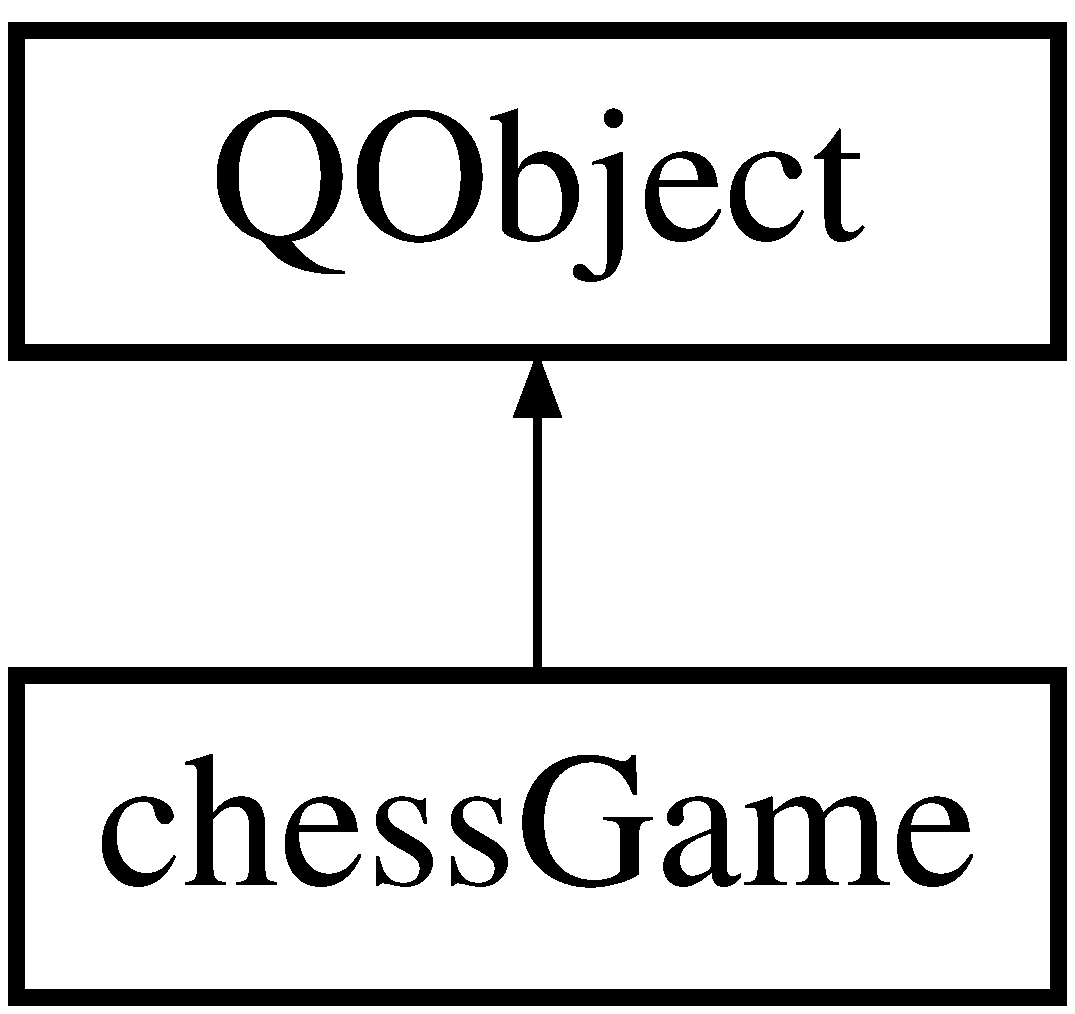
\includegraphics[height=2.000000cm]{classchess_game}
\end{center}
\end{figure}
\subsection*{Сигналы}
\begin{DoxyCompactItemize}
\item 
void \hyperlink{classchess_game_a8c0d3a3a193aac0635d173b584c97bcd}{made\+Move} (\hyperlink{classboard_move}{board\+Move} bm)
\begin{DoxyCompactList}\small\item\em made\+Move -\/ Был совершен ход \end{DoxyCompactList}\end{DoxyCompactItemize}
\subsection*{Открытые члены}
\begin{DoxyCompactItemize}
\item 
\hypertarget{classchess_game_a1e6fc778faac96b97fd66af94baa3a49}{}{\bfseries chess\+Game} (Q\+Object $\ast$parent=nullptr)\label{classchess_game_a1e6fc778faac96b97fd66af94baa3a49}

\item 
\hyperlink{classchess_game_a3d92d77fbd1f6834e72b64d8a9472a96}{chess\+Game} (\hyperlink{classchess_player}{chess\+Player} $\ast$p1, \hyperlink{classchess_player}{chess\+Player} $\ast$p2)
\begin{DoxyCompactList}\small\item\em \hyperlink{classchess_game}{chess\+Game} -\/ конструктор для инициализации парой игроков \end{DoxyCompactList}\item 
\hypertarget{classchess_game_ab8015aeeb33def6b01df544d5de76c62}{}\hyperlink{classchess_game_ab8015aeeb33def6b01df544d5de76c62}{$\sim$chess\+Game} ()\label{classchess_game_ab8015aeeb33def6b01df544d5de76c62}

\begin{DoxyCompactList}\small\item\em $\sim$chess\+Game корректно разрушает объект \end{DoxyCompactList}\item 
\hypertarget{classchess_game_ac4434ee888280b15097641146900aedf}{}void \hyperlink{classchess_game_ac4434ee888280b15097641146900aedf}{new\+Game} ()\label{classchess_game_ac4434ee888280b15097641146900aedf}

\begin{DoxyCompactList}\small\item\em new\+Game -\/ запускает новую игру \end{DoxyCompactList}\item 
void \hyperlink{classchess_game_a7d444b87ac60a620f3ae3b03893478e1}{load\+Game} (const \hyperlink{classchess_game_state}{chess\+Game\+State} \&cgs)
\begin{DoxyCompactList}\small\item\em load\+Game -\/ загружает игру \end{DoxyCompactList}\item 
\hypertarget{classchess_game_aca8e8ecb362a1a21232e5221ad9f6870}{}void \hyperlink{classchess_game_aca8e8ecb362a1a21232e5221ad9f6870}{start\+Game} ()\label{classchess_game_aca8e8ecb362a1a21232e5221ad9f6870}

\begin{DoxyCompactList}\small\item\em start\+Game -\/ начинает новую партию \end{DoxyCompactList}\item 
\hyperlink{classchess_player}{chess\+Player} $\ast$ \hyperlink{classchess_game_ae818720664a4aaaad9654c63ee138c39}{get\+Player1} () const 
\begin{DoxyCompactList}\small\item\em get\+Player2 -\/ возвращает белого игрока \end{DoxyCompactList}\item 
\hyperlink{classchess_player}{chess\+Player} $\ast$ \hyperlink{classchess_game_abe4bece4c525cd770a8b8c455cd2b462}{get\+Player2} () const 
\begin{DoxyCompactList}\small\item\em get\+Player2 -\/ возвращает белого игрока \end{DoxyCompactList}\item 
\hyperlink{classchess_player}{chess\+Player} $\ast$ \hyperlink{classchess_game_a1c5a201d0868ad9002b8e2ee1be8476f}{get\+Current\+Player} () const 
\begin{DoxyCompactList}\small\item\em get\+Current\+Player -\/ возвращает текущего игрока \end{DoxyCompactList}\item 
\hyperlink{classchess_player}{chess\+Player} $\ast$ \hyperlink{classchess_game_a3c7f8d99a70c6bc579e11c7a80498b20}{get\+Inactive\+Player} () const 
\begin{DoxyCompactList}\small\item\em get\+Inactive\+Player -\/ возвращает противоположного игрока \end{DoxyCompactList}\item 
\hyperlink{classchess_game_state}{chess\+Game\+State} \hyperlink{classchess_game_aa63acf0a17cc89fcc0e7535a369ebca2}{get\+Sate} () const 
\begin{DoxyCompactList}\small\item\em get\+Sate -\/ получит описание игровой ситуации \end{DoxyCompactList}\item 
\hyperlink{classboard}{board} \hyperlink{classchess_game_ab217741c1342afad766efdc680b46712}{get\+Board} () const 
\begin{DoxyCompactList}\small\item\em get\+Board -\/ получить доску \end{DoxyCompactList}\item 
\hyperlink{classpiece_a0e121e5952345fd0e7014a8e6a1fbbda}{piece\+::color} \hyperlink{classchess_game_a78099d4054ffd3bca6de2290504712e4}{get\+Color} () const 
\begin{DoxyCompactList}\small\item\em get\+Color -\/ получить цвет текущего хода \end{DoxyCompactList}\item 
bool \hyperlink{classchess_game_a93374e1eee491081f54793b70563e0e9}{try\+Move} (const \hyperlink{classboard_move}{board\+Move} \&bm)
\begin{DoxyCompactList}\small\item\em try\+Move -\/ попытаться сделать ход \end{DoxyCompactList}\item 
\hypertarget{classchess_game_af9eb38dee7afe0e7adc56c1ad0057de2}{}void \hyperlink{classchess_game_af9eb38dee7afe0e7adc56c1ad0057de2}{undo\+Move} ()\label{classchess_game_af9eb38dee7afe0e7adc56c1ad0057de2}

\begin{DoxyCompactList}\small\item\em undo\+Move -\/ отменяет последний ход \end{DoxyCompactList}\item 
bool \hyperlink{classchess_game_a139815c8ee6aa7ba7e6408cdf4e82edc}{can\+Cur} (const \hyperlink{classboard_position}{board\+Position} \&bp) const 
\begin{DoxyCompactList}\small\item\em can\+Cur -\/ можно ли использовать эту позицию для начала хода \end{DoxyCompactList}\end{DoxyCompactItemize}


\subsection{Подробное описание}
The \hyperlink{classchess_game}{chess\+Game} class -\/ класс партии 

\subsection{Конструктор(ы)}
\hypertarget{classchess_game_a3d92d77fbd1f6834e72b64d8a9472a96}{}\index{chess\+Game@{chess\+Game}!chess\+Game@{chess\+Game}}
\index{chess\+Game@{chess\+Game}!chess\+Game@{chess\+Game}}
\subsubsection[{chess\+Game}]{\setlength{\rightskip}{0pt plus 5cm}chess\+Game\+::chess\+Game (
\begin{DoxyParamCaption}
\item[{{\bf chess\+Player} $\ast$}]{p1, }
\item[{{\bf chess\+Player} $\ast$}]{p2}
\end{DoxyParamCaption}
)}\label{classchess_game_a3d92d77fbd1f6834e72b64d8a9472a96}


\hyperlink{classchess_game}{chess\+Game} -\/ конструктор для инициализации парой игроков 


\begin{DoxyParams}{Аргументы}
{\em p1} & -\/ белый игрок \\
\hline
{\em p2} & -\/ черный игрок \\
\hline
\end{DoxyParams}


\subsection{Методы}
\hypertarget{classchess_game_a139815c8ee6aa7ba7e6408cdf4e82edc}{}\index{chess\+Game@{chess\+Game}!can\+Cur@{can\+Cur}}
\index{can\+Cur@{can\+Cur}!chess\+Game@{chess\+Game}}
\subsubsection[{can\+Cur}]{\setlength{\rightskip}{0pt plus 5cm}bool chess\+Game\+::can\+Cur (
\begin{DoxyParamCaption}
\item[{const {\bf board\+Position} \&}]{bp}
\end{DoxyParamCaption}
) const\hspace{0.3cm}{\ttfamily [inline]}}\label{classchess_game_a139815c8ee6aa7ba7e6408cdf4e82edc}


can\+Cur -\/ можно ли использовать эту позицию для начала хода 


\begin{DoxyParams}{Аргументы}
{\em bp} & -\/ позиция \\
\hline
\end{DoxyParams}
\begin{DoxyReturn}{Возвращает}
-\/ можо или нет 
\end{DoxyReturn}
\hypertarget{classchess_game_ab217741c1342afad766efdc680b46712}{}\index{chess\+Game@{chess\+Game}!get\+Board@{get\+Board}}
\index{get\+Board@{get\+Board}!chess\+Game@{chess\+Game}}
\subsubsection[{get\+Board}]{\setlength{\rightskip}{0pt plus 5cm}{\bf board} chess\+Game\+::get\+Board (
\begin{DoxyParamCaption}
{}
\end{DoxyParamCaption}
) const\hspace{0.3cm}{\ttfamily [inline]}}\label{classchess_game_ab217741c1342afad766efdc680b46712}


get\+Board -\/ получить доску 

\begin{DoxyReturn}{Возвращает}
-\/ доска 
\end{DoxyReturn}
\hypertarget{classchess_game_a78099d4054ffd3bca6de2290504712e4}{}\index{chess\+Game@{chess\+Game}!get\+Color@{get\+Color}}
\index{get\+Color@{get\+Color}!chess\+Game@{chess\+Game}}
\subsubsection[{get\+Color}]{\setlength{\rightskip}{0pt plus 5cm}{\bf piece\+::color} chess\+Game\+::get\+Color (
\begin{DoxyParamCaption}
{}
\end{DoxyParamCaption}
) const\hspace{0.3cm}{\ttfamily [inline]}}\label{classchess_game_a78099d4054ffd3bca6de2290504712e4}


get\+Color -\/ получить цвет текущего хода 

\begin{DoxyReturn}{Возвращает}
цвет 
\end{DoxyReturn}
\hypertarget{classchess_game_a1c5a201d0868ad9002b8e2ee1be8476f}{}\index{chess\+Game@{chess\+Game}!get\+Current\+Player@{get\+Current\+Player}}
\index{get\+Current\+Player@{get\+Current\+Player}!chess\+Game@{chess\+Game}}
\subsubsection[{get\+Current\+Player}]{\setlength{\rightskip}{0pt plus 5cm}{\bf chess\+Player}$\ast$ chess\+Game\+::get\+Current\+Player (
\begin{DoxyParamCaption}
{}
\end{DoxyParamCaption}
) const\hspace{0.3cm}{\ttfamily [inline]}}\label{classchess_game_a1c5a201d0868ad9002b8e2ee1be8476f}


get\+Current\+Player -\/ возвращает текущего игрока 

\begin{DoxyReturn}{Возвращает}
-\/ указатель на игрока 
\end{DoxyReturn}
\hypertarget{classchess_game_a3c7f8d99a70c6bc579e11c7a80498b20}{}\index{chess\+Game@{chess\+Game}!get\+Inactive\+Player@{get\+Inactive\+Player}}
\index{get\+Inactive\+Player@{get\+Inactive\+Player}!chess\+Game@{chess\+Game}}
\subsubsection[{get\+Inactive\+Player}]{\setlength{\rightskip}{0pt plus 5cm}{\bf chess\+Player}$\ast$ chess\+Game\+::get\+Inactive\+Player (
\begin{DoxyParamCaption}
{}
\end{DoxyParamCaption}
) const\hspace{0.3cm}{\ttfamily [inline]}}\label{classchess_game_a3c7f8d99a70c6bc579e11c7a80498b20}


get\+Inactive\+Player -\/ возвращает противоположного игрока 

\begin{DoxyReturn}{Возвращает}
-\/ указатель на игрока 
\end{DoxyReturn}
\hypertarget{classchess_game_ae818720664a4aaaad9654c63ee138c39}{}\index{chess\+Game@{chess\+Game}!get\+Player1@{get\+Player1}}
\index{get\+Player1@{get\+Player1}!chess\+Game@{chess\+Game}}
\subsubsection[{get\+Player1}]{\setlength{\rightskip}{0pt plus 5cm}{\bf chess\+Player}$\ast$ chess\+Game\+::get\+Player1 (
\begin{DoxyParamCaption}
{}
\end{DoxyParamCaption}
) const\hspace{0.3cm}{\ttfamily [inline]}}\label{classchess_game_ae818720664a4aaaad9654c63ee138c39}


get\+Player2 -\/ возвращает белого игрока 

\begin{DoxyReturn}{Возвращает}
-\/ указатель на игрока 
\end{DoxyReturn}
\hypertarget{classchess_game_abe4bece4c525cd770a8b8c455cd2b462}{}\index{chess\+Game@{chess\+Game}!get\+Player2@{get\+Player2}}
\index{get\+Player2@{get\+Player2}!chess\+Game@{chess\+Game}}
\subsubsection[{get\+Player2}]{\setlength{\rightskip}{0pt plus 5cm}{\bf chess\+Player}$\ast$ chess\+Game\+::get\+Player2 (
\begin{DoxyParamCaption}
{}
\end{DoxyParamCaption}
) const\hspace{0.3cm}{\ttfamily [inline]}}\label{classchess_game_abe4bece4c525cd770a8b8c455cd2b462}


get\+Player2 -\/ возвращает белого игрока 

\begin{DoxyReturn}{Возвращает}
-\/ указатель на игрока 
\end{DoxyReturn}
\hypertarget{classchess_game_aa63acf0a17cc89fcc0e7535a369ebca2}{}\index{chess\+Game@{chess\+Game}!get\+Sate@{get\+Sate}}
\index{get\+Sate@{get\+Sate}!chess\+Game@{chess\+Game}}
\subsubsection[{get\+Sate}]{\setlength{\rightskip}{0pt plus 5cm}{\bf chess\+Game\+State} chess\+Game\+::get\+Sate (
\begin{DoxyParamCaption}
{}
\end{DoxyParamCaption}
) const\hspace{0.3cm}{\ttfamily [inline]}}\label{classchess_game_aa63acf0a17cc89fcc0e7535a369ebca2}


get\+Sate -\/ получит описание игровой ситуации 

\begin{DoxyReturn}{Возвращает}
-\/ ситуация 
\end{DoxyReturn}
\hypertarget{classchess_game_a7d444b87ac60a620f3ae3b03893478e1}{}\index{chess\+Game@{chess\+Game}!load\+Game@{load\+Game}}
\index{load\+Game@{load\+Game}!chess\+Game@{chess\+Game}}
\subsubsection[{load\+Game}]{\setlength{\rightskip}{0pt plus 5cm}void chess\+Game\+::load\+Game (
\begin{DoxyParamCaption}
\item[{const {\bf chess\+Game\+State} \&}]{cgs}
\end{DoxyParamCaption}
)}\label{classchess_game_a7d444b87ac60a620f3ae3b03893478e1}


load\+Game -\/ загружает игру 


\begin{DoxyParams}{Аргументы}
{\em cgs} & -\/ состояние игры \\
\hline
\end{DoxyParams}
\hypertarget{classchess_game_a8c0d3a3a193aac0635d173b584c97bcd}{}\index{chess\+Game@{chess\+Game}!made\+Move@{made\+Move}}
\index{made\+Move@{made\+Move}!chess\+Game@{chess\+Game}}
\subsubsection[{made\+Move}]{\setlength{\rightskip}{0pt plus 5cm}void chess\+Game\+::made\+Move (
\begin{DoxyParamCaption}
\item[{{\bf board\+Move}}]{bm}
\end{DoxyParamCaption}
)\hspace{0.3cm}{\ttfamily [signal]}}\label{classchess_game_a8c0d3a3a193aac0635d173b584c97bcd}


made\+Move -\/ Был совершен ход 


\begin{DoxyParams}{Аргументы}
{\em bm} & -\/ Ход который был совершен \\
\hline
\end{DoxyParams}
\hypertarget{classchess_game_a93374e1eee491081f54793b70563e0e9}{}\index{chess\+Game@{chess\+Game}!try\+Move@{try\+Move}}
\index{try\+Move@{try\+Move}!chess\+Game@{chess\+Game}}
\subsubsection[{try\+Move}]{\setlength{\rightskip}{0pt plus 5cm}bool chess\+Game\+::try\+Move (
\begin{DoxyParamCaption}
\item[{const {\bf board\+Move} \&}]{bm}
\end{DoxyParamCaption}
)}\label{classchess_game_a93374e1eee491081f54793b70563e0e9}


try\+Move -\/ попытаться сделать ход 


\begin{DoxyParams}{Аргументы}
{\em bm} & -\/ ход \\
\hline
\end{DoxyParams}
\begin{DoxyReturn}{Возвращает}
-\/ успешность попытки 
\end{DoxyReturn}


Объявления и описания членов классов находятся в файлах\+:\begin{DoxyCompactItemize}
\item 
Model/chessgame.\+h\item 
Model/chessgame.\+cpp\end{DoxyCompactItemize}

\hypertarget{classchess_game_state}{}\section{Класс chess\+Game\+State}
\label{classchess_game_state}\index{chess\+Game\+State@{chess\+Game\+State}}


The \hyperlink{classchess_game_state}{chess\+Game\+State} class -\/ класс описывающий игровое соостояние  




{\ttfamily \#include $<$chessgamestate.\+h$>$}

\subsection*{Открытые члены}
\begin{DoxyCompactItemize}
\item 
\hypertarget{classchess_game_state_a6cc0b8ba1e92e19ad235d1604ce3ff81}{}void \hyperlink{classchess_game_state_a6cc0b8ba1e92e19ad235d1604ce3ff81}{init} ()\label{classchess_game_state_a6cc0b8ba1e92e19ad235d1604ce3ff81}

\begin{DoxyCompactList}\small\item\em init -\/ приводит игровую статистику к стартовому состаянию \end{DoxyCompactList}\item 
void \hyperlink{classchess_game_state_a259cdc59bd56b6e9737d7d904a044cdd}{make\+Move} (const \hyperlink{classboard_move}{board\+Move} \&bm)
\begin{DoxyCompactList}\small\item\em make\+Move -\/ сделать ход \end{DoxyCompactList}\item 
\hyperlink{classboard}{board} \hyperlink{classchess_game_state_a711c3cf730b86934e2a194d34c0c5e16}{get\+Board} () const 
\begin{DoxyCompactList}\small\item\em get\+Board -\/ получить доску \end{DoxyCompactList}\item 
\hyperlink{classboard_move}{board\+Move} \hyperlink{classchess_game_state_af5b0dd9ad83beea6da4c951e0d09af03}{get\+Last\+Move} () const 
\begin{DoxyCompactList}\small\item\em get\+Last\+Move -\/ получить последний совершенный ход \end{DoxyCompactList}\item 
int \hyperlink{classchess_game_state_a49be350f4b7e8a10dab2ceff8753f529}{get\+Step\+Number} () const 
\begin{DoxyCompactList}\small\item\em get\+Step\+Number -\/ получить номер хода \end{DoxyCompactList}\item 
bool \hyperlink{classchess_game_state_a29925a54a671e3bb3bd51d1a87eb00ed}{is\+Chek} () const 
\begin{DoxyCompactList}\small\item\em is\+Chek -\/ шах на доске \end{DoxyCompactList}\item 
bool \hyperlink{classchess_game_state_a70098682d6f3a2cad6b2ac1832ae99c2}{is\+White\+Step} () const 
\begin{DoxyCompactList}\small\item\em is\+White\+Step -\/ какой цвет сходил в последний раз \end{DoxyCompactList}\item 
\hyperlink{classpiece_a0e121e5952345fd0e7014a8e6a1fbbda}{piece\+::color} \hyperlink{classchess_game_state_ab5011f008dbf3c7bc991a17edc4ceac1}{get\+Color} () const 
\begin{DoxyCompactList}\small\item\em get\+Color -\/ вернуть цвет хода \end{DoxyCompactList}\item 
bool \hyperlink{classchess_game_state_a2745c19291435d3fee468256b4f5c876}{is\+Position\+Selectable} (const \hyperlink{classboard_position}{board\+Position} \&bp) const 
\begin{DoxyCompactList}\small\item\em is\+Position\+Selectable -\/ можно ли эту клетку \end{DoxyCompactList}\end{DoxyCompactItemize}


\subsection{Подробное описание}
The \hyperlink{classchess_game_state}{chess\+Game\+State} class -\/ класс описывающий игровое соостояние 

\subsection{Методы}
\hypertarget{classchess_game_state_a711c3cf730b86934e2a194d34c0c5e16}{}\index{chess\+Game\+State@{chess\+Game\+State}!get\+Board@{get\+Board}}
\index{get\+Board@{get\+Board}!chess\+Game\+State@{chess\+Game\+State}}
\subsubsection[{get\+Board}]{\setlength{\rightskip}{0pt plus 5cm}{\bf board} chess\+Game\+State\+::get\+Board (
\begin{DoxyParamCaption}
{}
\end{DoxyParamCaption}
) const\hspace{0.3cm}{\ttfamily [inline]}}\label{classchess_game_state_a711c3cf730b86934e2a194d34c0c5e16}


get\+Board -\/ получить доску 

\begin{DoxyReturn}{Возвращает}
доска 
\end{DoxyReturn}
\hypertarget{classchess_game_state_ab5011f008dbf3c7bc991a17edc4ceac1}{}\index{chess\+Game\+State@{chess\+Game\+State}!get\+Color@{get\+Color}}
\index{get\+Color@{get\+Color}!chess\+Game\+State@{chess\+Game\+State}}
\subsubsection[{get\+Color}]{\setlength{\rightskip}{0pt plus 5cm}{\bf piece\+::color} chess\+Game\+State\+::get\+Color (
\begin{DoxyParamCaption}
{}
\end{DoxyParamCaption}
) const\hspace{0.3cm}{\ttfamily [inline]}}\label{classchess_game_state_ab5011f008dbf3c7bc991a17edc4ceac1}


get\+Color -\/ вернуть цвет хода 

\begin{DoxyReturn}{Возвращает}
цвет 
\end{DoxyReturn}
\hypertarget{classchess_game_state_af5b0dd9ad83beea6da4c951e0d09af03}{}\index{chess\+Game\+State@{chess\+Game\+State}!get\+Last\+Move@{get\+Last\+Move}}
\index{get\+Last\+Move@{get\+Last\+Move}!chess\+Game\+State@{chess\+Game\+State}}
\subsubsection[{get\+Last\+Move}]{\setlength{\rightskip}{0pt plus 5cm}{\bf board\+Move} chess\+Game\+State\+::get\+Last\+Move (
\begin{DoxyParamCaption}
{}
\end{DoxyParamCaption}
) const\hspace{0.3cm}{\ttfamily [inline]}}\label{classchess_game_state_af5b0dd9ad83beea6da4c951e0d09af03}


get\+Last\+Move -\/ получить последний совершенный ход 

\begin{DoxyReturn}{Возвращает}
-\/ ход 
\end{DoxyReturn}
\hypertarget{classchess_game_state_a49be350f4b7e8a10dab2ceff8753f529}{}\index{chess\+Game\+State@{chess\+Game\+State}!get\+Step\+Number@{get\+Step\+Number}}
\index{get\+Step\+Number@{get\+Step\+Number}!chess\+Game\+State@{chess\+Game\+State}}
\subsubsection[{get\+Step\+Number}]{\setlength{\rightskip}{0pt plus 5cm}int chess\+Game\+State\+::get\+Step\+Number (
\begin{DoxyParamCaption}
{}
\end{DoxyParamCaption}
) const\hspace{0.3cm}{\ttfamily [inline]}}\label{classchess_game_state_a49be350f4b7e8a10dab2ceff8753f529}


get\+Step\+Number -\/ получить номер хода 

\begin{DoxyReturn}{Возвращает}
номер хода 
\end{DoxyReturn}
\hypertarget{classchess_game_state_a29925a54a671e3bb3bd51d1a87eb00ed}{}\index{chess\+Game\+State@{chess\+Game\+State}!is\+Chek@{is\+Chek}}
\index{is\+Chek@{is\+Chek}!chess\+Game\+State@{chess\+Game\+State}}
\subsubsection[{is\+Chek}]{\setlength{\rightskip}{0pt plus 5cm}bool chess\+Game\+State\+::is\+Chek (
\begin{DoxyParamCaption}
{}
\end{DoxyParamCaption}
) const\hspace{0.3cm}{\ttfamily [inline]}}\label{classchess_game_state_a29925a54a671e3bb3bd51d1a87eb00ed}


is\+Chek -\/ шах на доске 

\begin{DoxyReturn}{Возвращает}
является ли положение шаховым 
\end{DoxyReturn}
\hypertarget{classchess_game_state_a2745c19291435d3fee468256b4f5c876}{}\index{chess\+Game\+State@{chess\+Game\+State}!is\+Position\+Selectable@{is\+Position\+Selectable}}
\index{is\+Position\+Selectable@{is\+Position\+Selectable}!chess\+Game\+State@{chess\+Game\+State}}
\subsubsection[{is\+Position\+Selectable}]{\setlength{\rightskip}{0pt plus 5cm}bool chess\+Game\+State\+::is\+Position\+Selectable (
\begin{DoxyParamCaption}
\item[{const {\bf board\+Position} \&}]{bp}
\end{DoxyParamCaption}
) const}\label{classchess_game_state_a2745c19291435d3fee468256b4f5c876}


is\+Position\+Selectable -\/ можно ли эту клетку 


\begin{DoxyParams}{Аргументы}
{\em bp} & -\/ позиция \\
\hline
\end{DoxyParams}
\begin{DoxyReturn}{Возвращает}
можно ли 
\end{DoxyReturn}
\hypertarget{classchess_game_state_a70098682d6f3a2cad6b2ac1832ae99c2}{}\index{chess\+Game\+State@{chess\+Game\+State}!is\+White\+Step@{is\+White\+Step}}
\index{is\+White\+Step@{is\+White\+Step}!chess\+Game\+State@{chess\+Game\+State}}
\subsubsection[{is\+White\+Step}]{\setlength{\rightskip}{0pt plus 5cm}bool chess\+Game\+State\+::is\+White\+Step (
\begin{DoxyParamCaption}
{}
\end{DoxyParamCaption}
) const\hspace{0.3cm}{\ttfamily [inline]}}\label{classchess_game_state_a70098682d6f3a2cad6b2ac1832ae99c2}


is\+White\+Step -\/ какой цвет сходил в последний раз 

\begin{DoxyReturn}{Возвращает}
-\/ был ли это белый цвет? 
\end{DoxyReturn}
\hypertarget{classchess_game_state_a259cdc59bd56b6e9737d7d904a044cdd}{}\index{chess\+Game\+State@{chess\+Game\+State}!make\+Move@{make\+Move}}
\index{make\+Move@{make\+Move}!chess\+Game\+State@{chess\+Game\+State}}
\subsubsection[{make\+Move}]{\setlength{\rightskip}{0pt plus 5cm}void chess\+Game\+State\+::make\+Move (
\begin{DoxyParamCaption}
\item[{const {\bf board\+Move} \&}]{bm}
\end{DoxyParamCaption}
)}\label{classchess_game_state_a259cdc59bd56b6e9737d7d904a044cdd}


make\+Move -\/ сделать ход 


\begin{DoxyParams}{Аргументы}
{\em bm} & -\/ ход \\
\hline
\end{DoxyParams}


Объявления и описания членов классов находятся в файлах\+:\begin{DoxyCompactItemize}
\item 
Model/chessgamestate.\+h\item 
Model/chessgamestate.\+cpp\end{DoxyCompactItemize}

\hypertarget{classchess_player}{}\section{Класс chess\+Player}
\label{classchess_player}\index{chess\+Player@{chess\+Player}}


The \hyperlink{classchess_player}{chess\+Player} class -\/ абстрактный класс игрока  




{\ttfamily \#include $<$chessplayer.\+h$>$}

Граф наследования\+:chess\+Player\+:\begin{figure}[H]
\begin{center}
\leavevmode
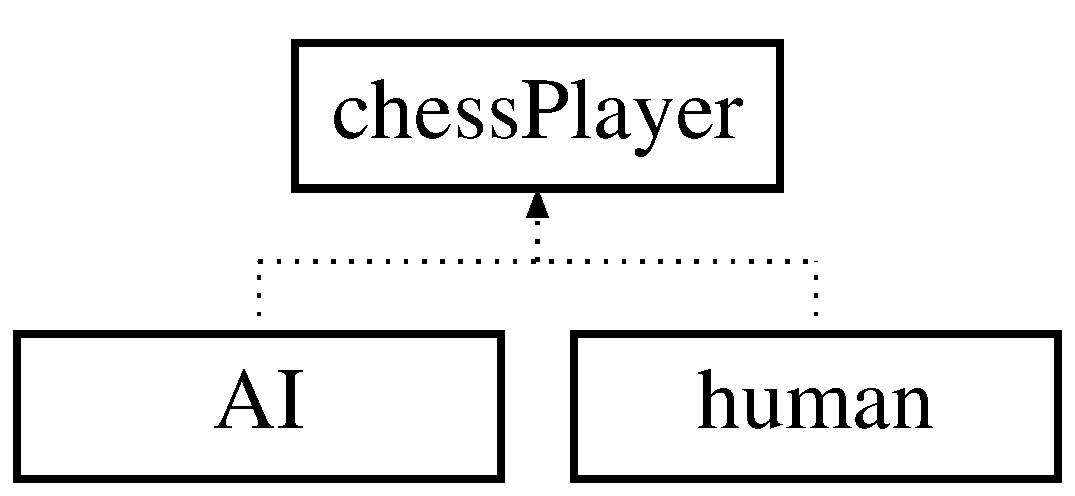
\includegraphics[height=2.000000cm]{classchess_player}
\end{center}
\end{figure}
\subsection*{Открытые члены}
\begin{DoxyCompactItemize}
\item 
\hypertarget{classchess_player_aa48ff4eddf1d46cbb989c0c00d779c83}{}virtual void {\bfseries new\+Game} ()=0\label{classchess_player_aa48ff4eddf1d46cbb989c0c00d779c83}

\item 
\hypertarget{classchess_player_a05e0031986866997afb0b861bda8f344}{}virtual void {\bfseries start\+Game} ()=0\label{classchess_player_a05e0031986866997afb0b861bda8f344}

\item 
\hypertarget{classchess_player_a0381db4f0afd40017762e9208eeff7b0}{}virtual void {\bfseries load\+Game} (const \hyperlink{classchess_game_state}{chess\+Game\+State} \&cgs)=0\label{classchess_player_a0381db4f0afd40017762e9208eeff7b0}

\item 
\hypertarget{classchess_player_acbb4583ddc816cf38b56d8c282aad412}{}virtual void {\bfseries opponent\+Move} (const \hyperlink{classboard_move}{board\+Move} \&move, const \hyperlink{classchess_game_state}{chess\+Game\+State} \&cgs)=0\label{classchess_player_acbb4583ddc816cf38b56d8c282aad412}

\item 
\hypertarget{classchess_player_a87501ca68fe97a4442f0e31e467c1820}{}bool {\bfseries is\+Thinking} () const \label{classchess_player_a87501ca68fe97a4442f0e31e467c1820}

\item 
\hypertarget{classchess_player_a0259369e1067e023a6f50f078a30cde3}{}bool {\bfseries is\+Human} () const \label{classchess_player_a0259369e1067e023a6f50f078a30cde3}

\item 
\hypertarget{classchess_player_aeed885d79b86767bc664f5f39c1b7df3}{}virtual void {\bfseries think} (const \hyperlink{classchess_game_state}{chess\+Game\+State} \&cgs)=0\label{classchess_player_aeed885d79b86767bc664f5f39c1b7df3}

\item 
\hypertarget{classchess_player_a55cdc430ded2d4c874bbd77a5c8d8f63}{}\hyperlink{classboard_move}{board\+Move} {\bfseries get\+Move} ()\label{classchess_player_a55cdc430ded2d4c874bbd77a5c8d8f63}

\item 
\hypertarget{classchess_player_a0e6d70cf9b9a52087055e755eb90532d}{}void {\bfseries interrupt\+Thinking} ()\label{classchess_player_a0e6d70cf9b9a52087055e755eb90532d}

\item 
\hypertarget{classchess_player_ad67bfb6b97ef3901d69b3ab86f0ee543}{}virtual bool {\bfseries need\+Move} ()=0\label{classchess_player_ad67bfb6b97ef3901d69b3ab86f0ee543}

\item 
\hypertarget{classchess_player_a34001badc8835ee50ba3cf7757bd5b49}{}void {\bfseries send\+Move} (const \hyperlink{classboard_move}{board\+Move} \&bm)\label{classchess_player_a34001badc8835ee50ba3cf7757bd5b49}

\item 
\hypertarget{classchess_player_ade3cee86e542229ac6475867afd8fdde}{}virtual void {\bfseries undo\+Move} ()=0\label{classchess_player_ade3cee86e542229ac6475867afd8fdde}

\item 
\hypertarget{classchess_player_aef6c947b54414da53ac4491e1f8488b7}{}void {\bfseries set\+Is\+White} (bool is\+White)\label{classchess_player_aef6c947b54414da53ac4491e1f8488b7}

\item 
\hypertarget{classchess_player_a7b2cb6f6e5c85185fc6ca5f74610eb70}{}bool {\bfseries is\+White} () const \label{classchess_player_a7b2cb6f6e5c85185fc6ca5f74610eb70}

\item 
\hypertarget{classchess_player_abe6500db94378533534d7bee0e7b9719}{}bool {\bfseries is\+Trustworthy} () const \label{classchess_player_abe6500db94378533534d7bee0e7b9719}

\item 
\hypertarget{classchess_player_a090b0e10bfcf88f98e4e28109b354947}{}\hyperlink{classpiece_a0e121e5952345fd0e7014a8e6a1fbbda}{piece\+::color} {\bfseries get\+Color} () const \label{classchess_player_a090b0e10bfcf88f98e4e28109b354947}

\end{DoxyCompactItemize}
\subsection*{Открытые статические члены}
\begin{DoxyCompactItemize}
\item 
\hypertarget{classchess_player_a9e9f6a9fb3e7a52bf8704afea2f8bd3e}{}static \hyperlink{classchess_player}{chess\+Player} $\ast$ {\bfseries create} (Q\+String type\+Name)\label{classchess_player_a9e9f6a9fb3e7a52bf8704afea2f8bd3e}

\end{DoxyCompactItemize}
\subsection*{Защищенные данные}
\begin{DoxyCompactItemize}
\item 
\hypertarget{classchess_player_a06252c21a45bb0b798b49f84a1d1dd5c}{}bool {\bfseries l\+Is\+White}\label{classchess_player_a06252c21a45bb0b798b49f84a1d1dd5c}

\item 
\hypertarget{classchess_player_aaeb0f6b585c49c7868040d96d8b9f297}{}bool {\bfseries l\+Is\+Thinking}\label{classchess_player_aaeb0f6b585c49c7868040d96d8b9f297}

\item 
\hypertarget{classchess_player_a566b824ad83a12cb505a48b2d4e1e4a4}{}bool {\bfseries l\+Is\+Human}\label{classchess_player_a566b824ad83a12cb505a48b2d4e1e4a4}

\item 
\hypertarget{classchess_player_aa282876d37f09361f03934fbc0cb5465}{}bool {\bfseries l\+Is\+Trustworthy}\label{classchess_player_aa282876d37f09361f03934fbc0cb5465}

\item 
\hypertarget{classchess_player_ac92aea6b6a84c5fd37c527fc22b441a2}{}\hyperlink{classboard_move}{board\+Move} {\bfseries l\+Move}\label{classchess_player_ac92aea6b6a84c5fd37c527fc22b441a2}

\end{DoxyCompactItemize}


\subsection{Подробное описание}
The \hyperlink{classchess_player}{chess\+Player} class -\/ абстрактный класс игрока 

Объявления и описания членов классов находятся в файлах\+:\begin{DoxyCompactItemize}
\item 
Model/chessplayer.\+h\item 
Model/chessplayer.\+cpp\end{DoxyCompactItemize}

\hypertarget{classhuman}{}\section{Класс human}
\label{classhuman}\index{human@{human}}


The human class -\/ описывает игрока человека  




{\ttfamily \#include $<$chessplayer.\+h$>$}

Граф наследования\+:human\+:\begin{figure}[H]
\begin{center}
\leavevmode
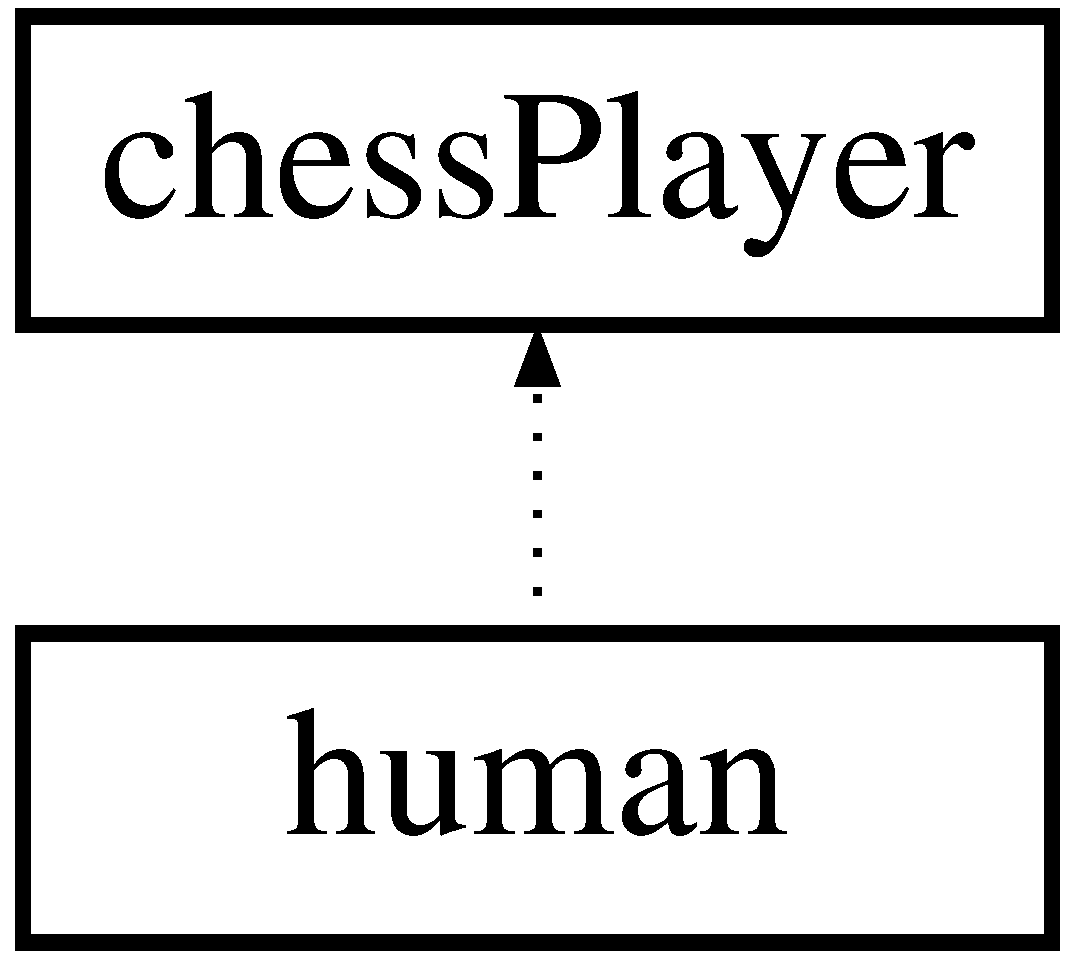
\includegraphics[height=2.000000cm]{classhuman}
\end{center}
\end{figure}
\subsection*{Открытые члены}
\begin{DoxyCompactItemize}
\item 
\hypertarget{classhuman_ab6ea3978f6ae2063a1d360d6e20a0b47}{}virtual void {\bfseries new\+Game} ()\label{classhuman_ab6ea3978f6ae2063a1d360d6e20a0b47}

\item 
\hypertarget{classhuman_abc8745ed5e64b8b310f0c76d2cbec5ae}{}virtual void {\bfseries start\+Game} ()\label{classhuman_abc8745ed5e64b8b310f0c76d2cbec5ae}

\item 
\hypertarget{classhuman_a1eb4181308ddcc845d1b343df3198571}{}virtual void {\bfseries load\+Game} (const \hyperlink{classchess_game_state}{chess\+Game\+State} \&cgs)\label{classhuman_a1eb4181308ddcc845d1b343df3198571}

\item 
\hypertarget{classhuman_a4f7c6fe7a7587988770a2bbdd958bdd8}{}virtual void {\bfseries opponent\+Move} (const \hyperlink{classboard_move}{board\+Move} \&move, const \hyperlink{classchess_game_state}{chess\+Game\+State} \&cgs)\label{classhuman_a4f7c6fe7a7587988770a2bbdd958bdd8}

\item 
\hypertarget{classhuman_ac6d7203ea1aed0d6d6f975fd6f742587}{}virtual void {\bfseries think} (const \hyperlink{classchess_game_state}{chess\+Game\+State} \&cgs)\label{classhuman_ac6d7203ea1aed0d6d6f975fd6f742587}

\item 
\hypertarget{classhuman_a9f4bf903965712cbf4eef040296a362c}{}virtual bool {\bfseries need\+Move} ()\label{classhuman_a9f4bf903965712cbf4eef040296a362c}

\item 
\hypertarget{classhuman_a7d61da059e3b85229206c9a16222e648}{}virtual void {\bfseries undo\+Move} ()\label{classhuman_a7d61da059e3b85229206c9a16222e648}

\end{DoxyCompactItemize}


\subsection{Подробное описание}
The human class -\/ описывает игрока человека 

Объявления и описания членов классов находятся в файлах\+:\begin{DoxyCompactItemize}
\item 
Model/chessplayer.\+h\item 
Model/chessplayer.\+cpp\end{DoxyCompactItemize}

\hypertarget{classoptions}{}\section{Класс options}
\label{classoptions}\index{options@{options}}


The options class -\/ класс конфигураций (содержит все конфигурации программы)  




{\ttfamily \#include $<$options.\+h$>$}

\subsection*{Открытые члены}
\begin{DoxyCompactItemize}
\item 
\hypertarget{classoptions_a41a256b4ba3b2d68a2d72b9245aa0c4d}{}\hyperlink{classoptions_a41a256b4ba3b2d68a2d72b9245aa0c4d}{options} ()\label{classoptions_a41a256b4ba3b2d68a2d72b9245aa0c4d}

\begin{DoxyCompactList}\small\item\em options -\/ Конструктор по умолчанию (в результате получается игра с параметрами по умолчанию) \end{DoxyCompactList}\item 
Q\+String \hyperlink{classoptions_aa08f770c27db29c587278cc0f8d3fb4d}{get\+Player1} () const 
\begin{DoxyCompactList}\small\item\em get\+Player1 -\/ Получить имя класса белого игрока \end{DoxyCompactList}\item 
Q\+String \hyperlink{classoptions_a26d94b8c314df0b355ba4f8dbf65eab5}{get\+Player2} () const 
\begin{DoxyCompactList}\small\item\em get\+Player2 -\/ Получить имя класса белого игрока \end{DoxyCompactList}\item 
Q\+Color \hyperlink{classoptions_aba7e46667f824c75d1acef548aeac3b4}{get\+Black\+Piece} () const 
\begin{DoxyCompactList}\small\item\em get\+Black\+Piece -\/ Получить цвет черных фигур \end{DoxyCompactList}\item 
Q\+Color \hyperlink{classoptions_a87429d553ea8c806f0f8623434c156a0}{get\+White\+Piece} () const 
\begin{DoxyCompactList}\small\item\em get\+White\+Piece -\/ Получить цвет белых фигур \end{DoxyCompactList}\item 
Q\+Color \hyperlink{classoptions_afa462be4a4c645b4cb616ae2d175b31c}{get\+Black\+Cell} () const 
\begin{DoxyCompactList}\small\item\em get\+Black\+Cell -\/ Получить цвет черных клеток \end{DoxyCompactList}\item 
Q\+Color \hyperlink{classoptions_a4297375082b4a84b4e350119254b3c85}{get\+White\+Cell} () const 
\begin{DoxyCompactList}\small\item\em get\+White\+Cell -\/ Получить цвет белых клеток \end{DoxyCompactList}\item 
Q\+Color \hyperlink{classoptions_ad26a5fdfdaf092c39ac3d167981bd2b5}{get\+Black\+Cell\+Attacked} () const 
\begin{DoxyCompactList}\small\item\em get\+Black\+Cell\+Attacked -\/ Получить цвет черных клеток во время атаки \end{DoxyCompactList}\item 
Q\+Color \hyperlink{classoptions_a95fa8aa7c9cbe5ee3a3e82f1bd0fdaee}{get\+White\+Cell\+Attacked} () const 
\begin{DoxyCompactList}\small\item\em get\+White\+Cell\+Attacked -\/ Получить цвет белых клеток во время атаки \end{DoxyCompactList}\item 
Q\+Color \hyperlink{classoptions_a95a5a628fa05ad2a3ca88f8cb4ef1d79}{get\+Black\+Cell\+Can\+Move} () const 
\begin{DoxyCompactList}\small\item\em get\+Black\+Cell\+Can\+Move -\/ Получить цвет черных клеток на которые можно сделать ход \end{DoxyCompactList}\item 
Q\+Color \hyperlink{classoptions_a609c97a120c62486181725426fe92a6b}{get\+White\+Cell\+Can\+Move} () const 
\begin{DoxyCompactList}\small\item\em get\+White\+Cell\+Can\+Move -\/ Получить цвет белых клеток на которые можно сделать ход \end{DoxyCompactList}\item 
Q\+Color \hyperlink{classoptions_a56556f6bdb79fd1ce44be18c7c10ed7f}{get\+Dead\+Cell} () const 
\begin{DoxyCompactList}\small\item\em get\+Black\+Piece -\/ Получить цвет клеток мертвых фигур \end{DoxyCompactList}\item 
int \hyperlink{classoptions_ab42e8a4fcf2d37c996cbe2f3158a8a72}{get\+Ai\+Cof1} () const 
\begin{DoxyCompactList}\small\item\em get\+Ai\+Cof1 -\/ получить коофициент сложности белого игрока \end{DoxyCompactList}\item 
int \hyperlink{classoptions_a401745de111fcebb990a4d365a237c72}{get\+Ai\+Cof2} () const 
\begin{DoxyCompactList}\small\item\em get\+Ai\+Cof1 -\/ получить коофициент сложности черного игрока \end{DoxyCompactList}\item 
void \hyperlink{classoptions_a148197ca3741db3a4117295a3705cbbc}{set\+Ai\+Cof1} (int c)
\begin{DoxyCompactList}\small\item\em set\+Ai\+Cof1 -\/ задать коофициент сложности белого игрока \end{DoxyCompactList}\item 
void \hyperlink{classoptions_a0ba88f307d3877a0c9c5b4fd71a30dab}{set\+Ai\+Cof2} (int c)
\begin{DoxyCompactList}\small\item\em set\+Ai\+Cof2 -\/ задать коофициент сложности белого игрока \end{DoxyCompactList}\item 
void \hyperlink{classoptions_a44dced3081a60094dfa7a010d7a77ab4}{set\+Player1} (Q\+String p)
\begin{DoxyCompactList}\small\item\em set\+Player1 -\/ задать тип белого игрока \end{DoxyCompactList}\item 
void \hyperlink{classoptions_a73da82a3067efd5a86bdc04f509570cb}{set\+Player2} (Q\+String p)
\begin{DoxyCompactList}\small\item\em set\+Player2 -\/ задать тип черного игрока \end{DoxyCompactList}\end{DoxyCompactItemize}


\subsection{Подробное описание}
The options class -\/ класс конфигураций (содержит все конфигурации программы) 

\subsection{Методы}
\hypertarget{classoptions_ab42e8a4fcf2d37c996cbe2f3158a8a72}{}\index{options@{options}!get\+Ai\+Cof1@{get\+Ai\+Cof1}}
\index{get\+Ai\+Cof1@{get\+Ai\+Cof1}!options@{options}}
\subsubsection[{get\+Ai\+Cof1}]{\setlength{\rightskip}{0pt plus 5cm}int options\+::get\+Ai\+Cof1 (
\begin{DoxyParamCaption}
{}
\end{DoxyParamCaption}
) const\hspace{0.3cm}{\ttfamily [inline]}}\label{classoptions_ab42e8a4fcf2d37c996cbe2f3158a8a72}


get\+Ai\+Cof1 -\/ получить коофициент сложности белого игрока 

\begin{DoxyReturn}{Возвращает}
коофициент от 1 до 3 
\end{DoxyReturn}
\hypertarget{classoptions_a401745de111fcebb990a4d365a237c72}{}\index{options@{options}!get\+Ai\+Cof2@{get\+Ai\+Cof2}}
\index{get\+Ai\+Cof2@{get\+Ai\+Cof2}!options@{options}}
\subsubsection[{get\+Ai\+Cof2}]{\setlength{\rightskip}{0pt plus 5cm}int options\+::get\+Ai\+Cof2 (
\begin{DoxyParamCaption}
{}
\end{DoxyParamCaption}
) const\hspace{0.3cm}{\ttfamily [inline]}}\label{classoptions_a401745de111fcebb990a4d365a237c72}


get\+Ai\+Cof1 -\/ получить коофициент сложности черного игрока 

\begin{DoxyReturn}{Возвращает}
коофициент от 1 до 3 
\end{DoxyReturn}
\hypertarget{classoptions_afa462be4a4c645b4cb616ae2d175b31c}{}\index{options@{options}!get\+Black\+Cell@{get\+Black\+Cell}}
\index{get\+Black\+Cell@{get\+Black\+Cell}!options@{options}}
\subsubsection[{get\+Black\+Cell}]{\setlength{\rightskip}{0pt plus 5cm}Q\+Color options\+::get\+Black\+Cell (
\begin{DoxyParamCaption}
{}
\end{DoxyParamCaption}
) const\hspace{0.3cm}{\ttfamily [inline]}}\label{classoptions_afa462be4a4c645b4cb616ae2d175b31c}


get\+Black\+Cell -\/ Получить цвет черных клеток 

\begin{DoxyReturn}{Возвращает}
цвет 
\end{DoxyReturn}
\hypertarget{classoptions_ad26a5fdfdaf092c39ac3d167981bd2b5}{}\index{options@{options}!get\+Black\+Cell\+Attacked@{get\+Black\+Cell\+Attacked}}
\index{get\+Black\+Cell\+Attacked@{get\+Black\+Cell\+Attacked}!options@{options}}
\subsubsection[{get\+Black\+Cell\+Attacked}]{\setlength{\rightskip}{0pt plus 5cm}Q\+Color options\+::get\+Black\+Cell\+Attacked (
\begin{DoxyParamCaption}
{}
\end{DoxyParamCaption}
) const\hspace{0.3cm}{\ttfamily [inline]}}\label{classoptions_ad26a5fdfdaf092c39ac3d167981bd2b5}


get\+Black\+Cell\+Attacked -\/ Получить цвет черных клеток во время атаки 

\begin{DoxyReturn}{Возвращает}
цвет 
\end{DoxyReturn}
\hypertarget{classoptions_a95a5a628fa05ad2a3ca88f8cb4ef1d79}{}\index{options@{options}!get\+Black\+Cell\+Can\+Move@{get\+Black\+Cell\+Can\+Move}}
\index{get\+Black\+Cell\+Can\+Move@{get\+Black\+Cell\+Can\+Move}!options@{options}}
\subsubsection[{get\+Black\+Cell\+Can\+Move}]{\setlength{\rightskip}{0pt plus 5cm}Q\+Color options\+::get\+Black\+Cell\+Can\+Move (
\begin{DoxyParamCaption}
{}
\end{DoxyParamCaption}
) const\hspace{0.3cm}{\ttfamily [inline]}}\label{classoptions_a95a5a628fa05ad2a3ca88f8cb4ef1d79}


get\+Black\+Cell\+Can\+Move -\/ Получить цвет черных клеток на которые можно сделать ход 

\begin{DoxyReturn}{Возвращает}
цвет 
\end{DoxyReturn}
\hypertarget{classoptions_aba7e46667f824c75d1acef548aeac3b4}{}\index{options@{options}!get\+Black\+Piece@{get\+Black\+Piece}}
\index{get\+Black\+Piece@{get\+Black\+Piece}!options@{options}}
\subsubsection[{get\+Black\+Piece}]{\setlength{\rightskip}{0pt plus 5cm}Q\+Color options\+::get\+Black\+Piece (
\begin{DoxyParamCaption}
{}
\end{DoxyParamCaption}
) const\hspace{0.3cm}{\ttfamily [inline]}}\label{classoptions_aba7e46667f824c75d1acef548aeac3b4}


get\+Black\+Piece -\/ Получить цвет черных фигур 

\begin{DoxyReturn}{Возвращает}
цвет 
\end{DoxyReturn}
\hypertarget{classoptions_a56556f6bdb79fd1ce44be18c7c10ed7f}{}\index{options@{options}!get\+Dead\+Cell@{get\+Dead\+Cell}}
\index{get\+Dead\+Cell@{get\+Dead\+Cell}!options@{options}}
\subsubsection[{get\+Dead\+Cell}]{\setlength{\rightskip}{0pt plus 5cm}Q\+Color options\+::get\+Dead\+Cell (
\begin{DoxyParamCaption}
{}
\end{DoxyParamCaption}
) const\hspace{0.3cm}{\ttfamily [inline]}}\label{classoptions_a56556f6bdb79fd1ce44be18c7c10ed7f}


get\+Black\+Piece -\/ Получить цвет клеток мертвых фигур 

\begin{DoxyReturn}{Возвращает}
цвет 
\end{DoxyReturn}
\hypertarget{classoptions_aa08f770c27db29c587278cc0f8d3fb4d}{}\index{options@{options}!get\+Player1@{get\+Player1}}
\index{get\+Player1@{get\+Player1}!options@{options}}
\subsubsection[{get\+Player1}]{\setlength{\rightskip}{0pt plus 5cm}Q\+String options\+::get\+Player1 (
\begin{DoxyParamCaption}
{}
\end{DoxyParamCaption}
) const\hspace{0.3cm}{\ttfamily [inline]}}\label{classoptions_aa08f770c27db29c587278cc0f8d3fb4d}


get\+Player1 -\/ Получить имя класса белого игрока 

\begin{DoxyReturn}{Возвращает}
имя класса (Например\+: \char`\"{}\+A\+I\char`\"{} или \char`\"{}humen\char`\"{}); 
\end{DoxyReturn}
\hypertarget{classoptions_a26d94b8c314df0b355ba4f8dbf65eab5}{}\index{options@{options}!get\+Player2@{get\+Player2}}
\index{get\+Player2@{get\+Player2}!options@{options}}
\subsubsection[{get\+Player2}]{\setlength{\rightskip}{0pt plus 5cm}Q\+String options\+::get\+Player2 (
\begin{DoxyParamCaption}
{}
\end{DoxyParamCaption}
) const\hspace{0.3cm}{\ttfamily [inline]}}\label{classoptions_a26d94b8c314df0b355ba4f8dbf65eab5}


get\+Player2 -\/ Получить имя класса белого игрока 

\begin{DoxyReturn}{Возвращает}
имя класса (Например\+: \char`\"{}\+A\+I\char`\"{} или \char`\"{}humen\char`\"{}); 
\end{DoxyReturn}
\hypertarget{classoptions_a4297375082b4a84b4e350119254b3c85}{}\index{options@{options}!get\+White\+Cell@{get\+White\+Cell}}
\index{get\+White\+Cell@{get\+White\+Cell}!options@{options}}
\subsubsection[{get\+White\+Cell}]{\setlength{\rightskip}{0pt plus 5cm}Q\+Color options\+::get\+White\+Cell (
\begin{DoxyParamCaption}
{}
\end{DoxyParamCaption}
) const\hspace{0.3cm}{\ttfamily [inline]}}\label{classoptions_a4297375082b4a84b4e350119254b3c85}


get\+White\+Cell -\/ Получить цвет белых клеток 

\begin{DoxyReturn}{Возвращает}
цвет 
\end{DoxyReturn}
\hypertarget{classoptions_a95fa8aa7c9cbe5ee3a3e82f1bd0fdaee}{}\index{options@{options}!get\+White\+Cell\+Attacked@{get\+White\+Cell\+Attacked}}
\index{get\+White\+Cell\+Attacked@{get\+White\+Cell\+Attacked}!options@{options}}
\subsubsection[{get\+White\+Cell\+Attacked}]{\setlength{\rightskip}{0pt plus 5cm}Q\+Color options\+::get\+White\+Cell\+Attacked (
\begin{DoxyParamCaption}
{}
\end{DoxyParamCaption}
) const\hspace{0.3cm}{\ttfamily [inline]}}\label{classoptions_a95fa8aa7c9cbe5ee3a3e82f1bd0fdaee}


get\+White\+Cell\+Attacked -\/ Получить цвет белых клеток во время атаки 

\begin{DoxyReturn}{Возвращает}
цвет 
\end{DoxyReturn}
\hypertarget{classoptions_a609c97a120c62486181725426fe92a6b}{}\index{options@{options}!get\+White\+Cell\+Can\+Move@{get\+White\+Cell\+Can\+Move}}
\index{get\+White\+Cell\+Can\+Move@{get\+White\+Cell\+Can\+Move}!options@{options}}
\subsubsection[{get\+White\+Cell\+Can\+Move}]{\setlength{\rightskip}{0pt plus 5cm}Q\+Color options\+::get\+White\+Cell\+Can\+Move (
\begin{DoxyParamCaption}
{}
\end{DoxyParamCaption}
) const\hspace{0.3cm}{\ttfamily [inline]}}\label{classoptions_a609c97a120c62486181725426fe92a6b}


get\+White\+Cell\+Can\+Move -\/ Получить цвет белых клеток на которые можно сделать ход 

\begin{DoxyReturn}{Возвращает}
цвет 
\end{DoxyReturn}
\hypertarget{classoptions_a87429d553ea8c806f0f8623434c156a0}{}\index{options@{options}!get\+White\+Piece@{get\+White\+Piece}}
\index{get\+White\+Piece@{get\+White\+Piece}!options@{options}}
\subsubsection[{get\+White\+Piece}]{\setlength{\rightskip}{0pt plus 5cm}Q\+Color options\+::get\+White\+Piece (
\begin{DoxyParamCaption}
{}
\end{DoxyParamCaption}
) const\hspace{0.3cm}{\ttfamily [inline]}}\label{classoptions_a87429d553ea8c806f0f8623434c156a0}


get\+White\+Piece -\/ Получить цвет белых фигур 

\begin{DoxyReturn}{Возвращает}
цвет 
\end{DoxyReturn}
\hypertarget{classoptions_a148197ca3741db3a4117295a3705cbbc}{}\index{options@{options}!set\+Ai\+Cof1@{set\+Ai\+Cof1}}
\index{set\+Ai\+Cof1@{set\+Ai\+Cof1}!options@{options}}
\subsubsection[{set\+Ai\+Cof1}]{\setlength{\rightskip}{0pt plus 5cm}void options\+::set\+Ai\+Cof1 (
\begin{DoxyParamCaption}
\item[{int}]{c}
\end{DoxyParamCaption}
)\hspace{0.3cm}{\ttfamily [inline]}}\label{classoptions_a148197ca3741db3a4117295a3705cbbc}


set\+Ai\+Cof1 -\/ задать коофициент сложности белого игрока 


\begin{DoxyParams}{Аргументы}
{\em c} & -\/ коофициент от 1 до 3 \\
\hline
\end{DoxyParams}
\hypertarget{classoptions_a0ba88f307d3877a0c9c5b4fd71a30dab}{}\index{options@{options}!set\+Ai\+Cof2@{set\+Ai\+Cof2}}
\index{set\+Ai\+Cof2@{set\+Ai\+Cof2}!options@{options}}
\subsubsection[{set\+Ai\+Cof2}]{\setlength{\rightskip}{0pt plus 5cm}void options\+::set\+Ai\+Cof2 (
\begin{DoxyParamCaption}
\item[{int}]{c}
\end{DoxyParamCaption}
)\hspace{0.3cm}{\ttfamily [inline]}}\label{classoptions_a0ba88f307d3877a0c9c5b4fd71a30dab}


set\+Ai\+Cof2 -\/ задать коофициент сложности белого игрока 


\begin{DoxyParams}{Аргументы}
{\em c} & -\/ коофициент от 1 до 3 \\
\hline
\end{DoxyParams}
\hypertarget{classoptions_a44dced3081a60094dfa7a010d7a77ab4}{}\index{options@{options}!set\+Player1@{set\+Player1}}
\index{set\+Player1@{set\+Player1}!options@{options}}
\subsubsection[{set\+Player1}]{\setlength{\rightskip}{0pt plus 5cm}void options\+::set\+Player1 (
\begin{DoxyParamCaption}
\item[{Q\+String}]{p}
\end{DoxyParamCaption}
)\hspace{0.3cm}{\ttfamily [inline]}}\label{classoptions_a44dced3081a60094dfa7a010d7a77ab4}


set\+Player1 -\/ задать тип белого игрока 


\begin{DoxyParams}{Аргументы}
{\em p} & -\/ имя типа строкой \\
\hline
\end{DoxyParams}
\hypertarget{classoptions_a73da82a3067efd5a86bdc04f509570cb}{}\index{options@{options}!set\+Player2@{set\+Player2}}
\index{set\+Player2@{set\+Player2}!options@{options}}
\subsubsection[{set\+Player2}]{\setlength{\rightskip}{0pt plus 5cm}void options\+::set\+Player2 (
\begin{DoxyParamCaption}
\item[{Q\+String}]{p}
\end{DoxyParamCaption}
)\hspace{0.3cm}{\ttfamily [inline]}}\label{classoptions_a73da82a3067efd5a86bdc04f509570cb}


set\+Player2 -\/ задать тип черного игрока 


\begin{DoxyParams}{Аргументы}
{\em p} & -\/ имя типа строкой \\
\hline
\end{DoxyParams}


Объявления и описания членов классов находятся в файлах\+:\begin{DoxyCompactItemize}
\item 
Model/options.\+h\item 
Model/options.\+cpp\end{DoxyCompactItemize}

\hypertarget{classpiece}{}\section{Класс piece}
\label{classpiece}\index{piece@{piece}}


The piece class -\/ класс шахматной фигуры  




{\ttfamily \#include $<$piece.\+h$>$}

\subsection*{Открытые типы}
\begin{DoxyCompactItemize}
\item 
\hypertarget{classpiece_a60bdcec91f595c164fe08c6705f192d0}{}enum \hyperlink{classpiece_a60bdcec91f595c164fe08c6705f192d0}{type} \{ \\*
{\bfseries P\+A\+W\+N}, 
{\bfseries R\+O\+O\+K}, 
{\bfseries K\+N\+I\+G\+H\+T}, 
{\bfseries B\+I\+S\+H\+O\+P}, 
\\*
{\bfseries Q\+U\+E\+E\+N}, 
{\bfseries K\+I\+N\+G}, 
{\bfseries N\+O\+T\+Y\+P\+E}
 \}\label{classpiece_a60bdcec91f595c164fe08c6705f192d0}

\begin{DoxyCompactList}\small\item\em The type enum -\/ типы фигур \end{DoxyCompactList}\item 
\hypertarget{classpiece_a0e121e5952345fd0e7014a8e6a1fbbda}{}enum \hyperlink{classpiece_a0e121e5952345fd0e7014a8e6a1fbbda}{color} \{ {\bfseries B\+L\+A\+C\+K}, 
{\bfseries W\+H\+I\+T\+E}, 
{\bfseries N\+O\+C\+O\+L\+O\+R}
 \}\label{classpiece_a0e121e5952345fd0e7014a8e6a1fbbda}

\begin{DoxyCompactList}\small\item\em The сolor enum -\/ цвета фигур \end{DoxyCompactList}\end{DoxyCompactItemize}
\subsection*{Открытые члены}
\begin{DoxyCompactItemize}
\item 
\hyperlink{classpiece_ab950ed5525196aa83c59cfe04f5891db}{piece} (\hyperlink{classpiece_a0e121e5952345fd0e7014a8e6a1fbbda}{piece\+::color} c, \hyperlink{classpiece_a60bdcec91f595c164fe08c6705f192d0}{type} t)
\begin{DoxyCompactList}\small\item\em piece -\/ конструктор \end{DoxyCompactList}\item 
\hyperlink{classpiece_a0e121e5952345fd0e7014a8e6a1fbbda}{color} \hyperlink{classpiece_a71cc356d37aaadad54d0c20714a4f407}{get\+Color} () const 
\begin{DoxyCompactList}\small\item\em get\+Color -\/ вернуть цвет \end{DoxyCompactList}\item 
\hyperlink{classpiece_a60bdcec91f595c164fe08c6705f192d0}{type} \hyperlink{classpiece_a60c80dd266bdd0a51df294263ee639d4}{get\+Type} () const 
\begin{DoxyCompactList}\small\item\em get\+Type -\/ вернуть тип \end{DoxyCompactList}\item 
\hypertarget{classpiece_a72b1969c42c8fa89f41cb8c54b2438c3}{}void \hyperlink{classpiece_a72b1969c42c8fa89f41cb8c54b2438c3}{clear\+State} ()\label{classpiece_a72b1969c42c8fa89f41cb8c54b2438c3}

\begin{DoxyCompactList}\small\item\em clear\+State -\/ отчистка статистики \end{DoxyCompactList}\item 
void \hyperlink{classpiece_a4771f62c2b12989f5051d7e96387159f}{turn\+Pawn\+To\+Other\+Piece} (\hyperlink{classpiece_a60bdcec91f595c164fe08c6705f192d0}{type} t)
\begin{DoxyCompactList}\small\item\em turn\+Pawn\+To\+Other\+Piece -\/ превращает пешку в фигуру с заданным типом кроме короля \end{DoxyCompactList}\end{DoxyCompactItemize}
\subsection*{Открытые статические члены}
\begin{DoxyCompactItemize}
\item 
static \hyperlink{classpiece_a0e121e5952345fd0e7014a8e6a1fbbda}{color} \hyperlink{classpiece_abc6324159644ab0c0aad7f2c84e122e5}{opponent\+Color} (\hyperlink{classpiece_a0e121e5952345fd0e7014a8e6a1fbbda}{color} c)
\begin{DoxyCompactList}\small\item\em opponent\+Color -\/ возвращает противоположный цвет \end{DoxyCompactList}\end{DoxyCompactItemize}
\subsection*{Защищенные данные}
\begin{DoxyCompactItemize}
\item 
\hypertarget{classpiece_a454fc10cb5287d35c1cea5890061ce41}{}\hyperlink{classpiece_a60bdcec91f595c164fe08c6705f192d0}{type} \hyperlink{classpiece_a454fc10cb5287d35c1cea5890061ce41}{l\+Type}\label{classpiece_a454fc10cb5287d35c1cea5890061ce41}

\begin{DoxyCompactList}\small\item\em l\+Type -\/ Тип фигуры \end{DoxyCompactList}\item 
\hypertarget{classpiece_a8a250da59070e11f3e301c623afffac6}{}\hyperlink{classpiece_a0e121e5952345fd0e7014a8e6a1fbbda}{color} \hyperlink{classpiece_a8a250da59070e11f3e301c623afffac6}{l\+Color}\label{classpiece_a8a250da59070e11f3e301c623afffac6}

\begin{DoxyCompactList}\small\item\em l\+Color -\/ Цвет фигуры \end{DoxyCompactList}\item 
\hypertarget{classpiece_afa0cccea76767519bb297420eb12bf1b}{}Q\+Stack$<$ \hyperlink{classstat_snapshot}{stat\+Snapshot} $>$ \hyperlink{classpiece_afa0cccea76767519bb297420eb12bf1b}{l\+Stat}\label{classpiece_afa0cccea76767519bb297420eb12bf1b}

\begin{DoxyCompactList}\small\item\em l\+Stat -\/ Хранит статистику \end{DoxyCompactList}\end{DoxyCompactItemize}


\subsection{Подробное описание}
The piece class -\/ класс шахматной фигуры 

\subsection{Конструктор(ы)}
\hypertarget{classpiece_ab950ed5525196aa83c59cfe04f5891db}{}\index{piece@{piece}!piece@{piece}}
\index{piece@{piece}!piece@{piece}}
\subsubsection[{piece}]{\setlength{\rightskip}{0pt plus 5cm}piece\+::piece (
\begin{DoxyParamCaption}
\item[{{\bf piece\+::color}}]{c, }
\item[{{\bf piece\+::type}}]{t}
\end{DoxyParamCaption}
)}\label{classpiece_ab950ed5525196aa83c59cfe04f5891db}


piece -\/ конструктор 


\begin{DoxyParams}{Аргументы}
{\em c} & -\/ цвет \\
\hline
{\em t} & -\/ тип \\
\hline
\end{DoxyParams}


\subsection{Методы}
\hypertarget{classpiece_a71cc356d37aaadad54d0c20714a4f407}{}\index{piece@{piece}!get\+Color@{get\+Color}}
\index{get\+Color@{get\+Color}!piece@{piece}}
\subsubsection[{get\+Color}]{\setlength{\rightskip}{0pt plus 5cm}{\bf color} piece\+::get\+Color (
\begin{DoxyParamCaption}
{}
\end{DoxyParamCaption}
) const\hspace{0.3cm}{\ttfamily [inline]}}\label{classpiece_a71cc356d37aaadad54d0c20714a4f407}


get\+Color -\/ вернуть цвет 

\begin{DoxyReturn}{Возвращает}
-\/цвет 
\end{DoxyReturn}
\hypertarget{classpiece_a60c80dd266bdd0a51df294263ee639d4}{}\index{piece@{piece}!get\+Type@{get\+Type}}
\index{get\+Type@{get\+Type}!piece@{piece}}
\subsubsection[{get\+Type}]{\setlength{\rightskip}{0pt plus 5cm}{\bf type} piece\+::get\+Type (
\begin{DoxyParamCaption}
{}
\end{DoxyParamCaption}
) const\hspace{0.3cm}{\ttfamily [inline]}}\label{classpiece_a60c80dd266bdd0a51df294263ee639d4}


get\+Type -\/ вернуть тип 

\begin{DoxyReturn}{Возвращает}
тип 
\end{DoxyReturn}
\hypertarget{classpiece_abc6324159644ab0c0aad7f2c84e122e5}{}\index{piece@{piece}!opponent\+Color@{opponent\+Color}}
\index{opponent\+Color@{opponent\+Color}!piece@{piece}}
\subsubsection[{opponent\+Color}]{\setlength{\rightskip}{0pt plus 5cm}static {\bf color} piece\+::opponent\+Color (
\begin{DoxyParamCaption}
\item[{{\bf color}}]{c}
\end{DoxyParamCaption}
)\hspace{0.3cm}{\ttfamily [inline]}, {\ttfamily [static]}}\label{classpiece_abc6324159644ab0c0aad7f2c84e122e5}


opponent\+Color -\/ возвращает противоположный цвет 


\begin{DoxyParams}{Аргументы}
{\em c} & -\/ цвет \\
\hline
\end{DoxyParams}
\begin{DoxyReturn}{Возвращает}
-\/ противоположный цвет 
\end{DoxyReturn}
\hypertarget{classpiece_a4771f62c2b12989f5051d7e96387159f}{}\index{piece@{piece}!turn\+Pawn\+To\+Other\+Piece@{turn\+Pawn\+To\+Other\+Piece}}
\index{turn\+Pawn\+To\+Other\+Piece@{turn\+Pawn\+To\+Other\+Piece}!piece@{piece}}
\subsubsection[{turn\+Pawn\+To\+Other\+Piece}]{\setlength{\rightskip}{0pt plus 5cm}void piece\+::turn\+Pawn\+To\+Other\+Piece (
\begin{DoxyParamCaption}
\item[{{\bf piece\+::type}}]{t}
\end{DoxyParamCaption}
)}\label{classpiece_a4771f62c2b12989f5051d7e96387159f}


turn\+Pawn\+To\+Other\+Piece -\/ превращает пешку в фигуру с заданным типом кроме короля 


\begin{DoxyParams}{Аргументы}
{\em t} & -\/ тип фигуры \\
\hline
\end{DoxyParams}


Объявления и описания членов классов находятся в файлах\+:\begin{DoxyCompactItemize}
\item 
Model/piece.\+h\item 
Model/piece.\+cpp\end{DoxyCompactItemize}

\hypertarget{classpiece_set}{}\section{Класс piece\+Set}
\label{classpiece_set}\index{piece\+Set@{piece\+Set}}


Объявления и описания членов классов находятся в файлах\+:\begin{DoxyCompactItemize}
\item 
Model/pieceset.\+h\item 
Model/pieceset.\+cpp\end{DoxyCompactItemize}

\hypertarget{structserial_board}{}\section{Структура serial\+Board}
\label{structserial_board}\index{serial\+Board@{serial\+Board}}


The \hyperlink{structserial_board}{serial\+Board} struct -\/ упращенная структура представления доски  




{\ttfamily \#include $<$board.\+h$>$}

\subsection*{Открытые атрибуты}
\begin{DoxyCompactItemize}
\item 
\hypertarget{structserial_board_a0a27eb05a8303039ae133c24c99e5665}{}mask {\bfseries pieces} \mbox{[}6\mbox{]}\label{structserial_board_a0a27eb05a8303039ae133c24c99e5665}

\item 
\hypertarget{structserial_board_a902c488370344e2ba5d48a64e3d4aa75}{}mask {\bfseries color} \mbox{[}2\mbox{]}\label{structserial_board_a902c488370344e2ba5d48a64e3d4aa75}

\item 
\hypertarget{structserial_board_a362750c1f255e200d28d4b2f34699c92}{}\begin{tabbing}
xx\=xx\=xx\=xx\=xx\=xx\=xx\=xx\=xx\=\kill
union \{\\
\>int {\bfseries allFlags}\\
\hypertarget{unionserial_board_1_1@0_a24409ca85bea9c6dab79a506c491785d}{}\>struct \{\\
\>\>int {\bfseries whiteEnpassant}:8\\
\>\>int {\bfseries blackEnpassant}:8\\
\>\>int {\bfseries whiteTurn}:1\\
\>\>int {\bfseries wkCastling}:1\\
\>\>int {\bfseries wqCastling}:1\\
\>\>int {\bfseries bkCastling}:1\\
\>\>int {\bfseries bqCastling}:1\\
\>\>int {\bfseries \_\_pad0\_\_}:11\\
\>\} \label{unionserial_board_1_1@0_a24409ca85bea9c6dab79a506c491785d}
\\
\}; \label{structserial_board_a362750c1f255e200d28d4b2f34699c92}
\\

\end{tabbing}\end{DoxyCompactItemize}


\subsection{Подробное описание}
The \hyperlink{structserial_board}{serial\+Board} struct -\/ упращенная структура представления доски 

Объявления и описания членов структуры находятся в файле\+:\begin{DoxyCompactItemize}
\item 
Model/board.\+h\end{DoxyCompactItemize}

\hypertarget{classstat_snapshot}{}\section{Класс stat\+Snapshot}
\label{classstat_snapshot}\index{stat\+Snapshot@{stat\+Snapshot}}


Объявления и описания членов классов находятся в файлах\+:\begin{DoxyCompactItemize}
\item 
Model/statsnapshot.\+h\item 
Model/statsnapshot.\+cpp\end{DoxyCompactItemize}

%--- End generated contents ---

% Index
\backmatter
\newpage
\phantomsection
\clearemptydoublepage
\addcontentsline{toc}{chapter}{Алфавитный указатель}
\printindex

\end{document}
